\documentclass[a4paper,12pt]{psar}

\usepackage{amsmath}
\usepackage{listings}
\usepackage{setspace}

% ---- PSAR Metadata ----
\projecttitle{Système de stockage distribué basé sur une DHT}
\projectsubtitle{Projet Master Systèmes et Applications Répartis (SAR)}
\projectcode{PSAR}

\authors{
  Cedric Genevieve,
  Safa Gunes,
  Somaya Boudalil\\
  Étudiants en Master 2026 — Systèmes et Applications Répartis
}

\Instructor{
  Prof.\ Alessio Pagliari
}

\institution{Sorbonne Université}
\projectdate{\today}

\begin{document}

\maketitlepage

\psarstartline
\tableofcontents
\vspace{1em}

\newpage

\section{Analyse Comparative des Paradigmes Architecturaux de Stockage Distribu\'e}

\setlength{\parskip}{3pt}

La croissance du volume de donn\'ees a rendu les architectures centralisees insuffisantes. Les systemes distribues sont devenus la norme, mais posent un defi central : garantir un \emph{lookup} efficace, la \emph{consistency} et la \emph{fault tolerance} dans un environnement de n\oe uds peu fiables.

Dans ce projet Master, nous comparons deux architectures de reference pour le stockage distribue, basees sur des paradigmes differents :

\paragraph{1. L'architecture P2P structur\'ee (Les DHTs)}
Paradigme decentralise (architecture \emph{symmetric}) : les n\oe uds ont un role homogene et s'auto-organisent dans un \emph{overlay} structure. Nous considerons plusieurs DHT (Chord, CAN, Pastry, Kademlia) qui resolvent le \emph{lookup} en general en $O(\log N)$, avec des compromis differents entre topologie logique, latence de routage, taille des tables d'etat et r\'esilience au \emph{churn}.

\paragraph{2. L'architecture hi\'erarchis\'ee orient\'ee colonnes (Mod\`ele HBase)}
A l'oppose du P2P pur, ce paradigme suit une architecture \emph{master-worker} inspiree de Bigtable. HBase vise une coherence forte, un modele oriente colonnes/versionne, et conserve une centralisation partielle (HMaster) pour la gestion des metadonnees et des transactions, en echange de meilleures performances d'ecriture et de scan.

La suite du document presente d'abord le routage et la maintenance des DHTs, puis l'architecture interne de HBase et ses mecanismes de persistance.

\subsection{\'Etude des approches P2P structur\'ee: Les DHTs}

Cette section r\'esume les principes essentiels des \emph{Distributed Hash Tables} (DHTs) : localisation des donn\'ees, routage, gestion des n\oe uds et interfaces applicatives.

\begin{tcolorbox}[bluebox]
\textbf{R\'ef\'erence} : \textcite{DBLP:conf/p2p/WehrleGR05}.
\end{tcolorbox}

\subsubsection{Introduction au probl\`eme du Lookup}

Le probl\`eme central est le \emph{lookup problem} : o\`u stocker une donn\'ee \(D\), puis comment la retrouver dans un r\'eseau distribu\'e sans coordination centrale.
\begin{quote}
\emph{"O\`u stocker, et comment trouver un certain \'el\'ement de donn\'ee D dans un syst\`eme distribu\'e sans aucun contr\^ole ou coordination centralis\'es ?"}
\end{quote}

\begin{figure}[!ht]
	\centering
		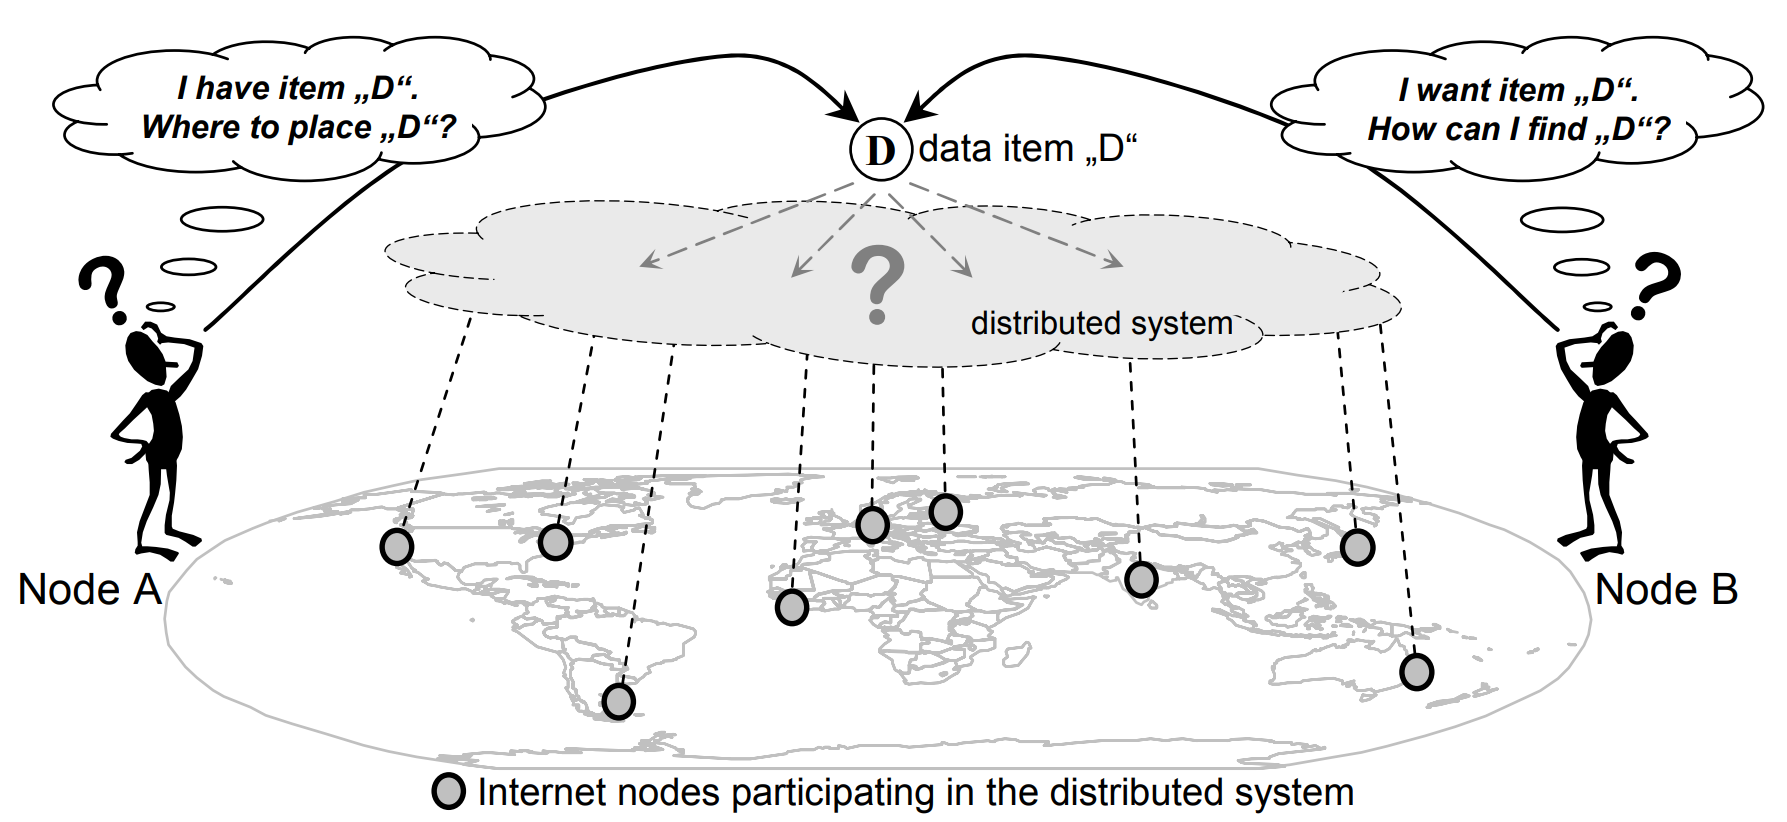
\includegraphics[width=0.7\textwidth]{images/00_lookup_problem.png}
	\caption{\textbf{Le probl\`eme du lookup} : le n\oe ud A stocke une donn\'ee \(D\) et le n\oe ud B doit la retrouver sans conna\^itre son emplacement.}
	\label{fig:00_lookup_problem}
\end{figure}

\newpage
\subsubsection{Comparaison des strat\'egies de recherche}

Trois familles de solutions sont compar\'ees.

\subsubsection*{1. Central Server}
Approche de \textbf{premi\`ere g\'en\'eration} (ex.~Napster). Un serveur central indexe les contenus. Recherche rapide en \(O(1)\), mais d\'ependance forte \`a un \emph{single point of failure}.

\begin{figure}[!ht]
	\centering
		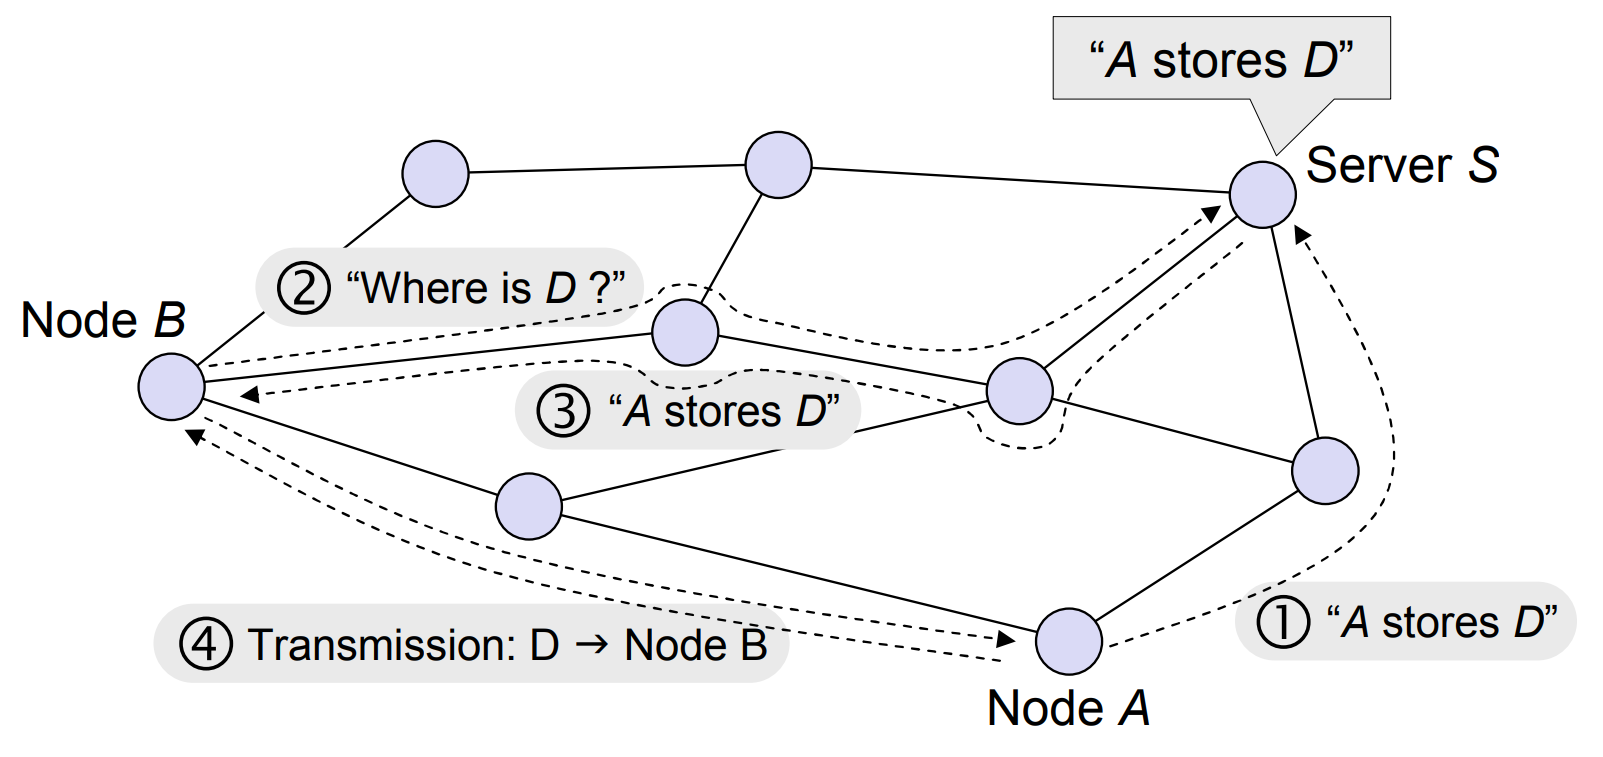
\includegraphics[width=0.7\textwidth]{images/01_central_server.png}
	\caption{\textbf{Central Server} : publication, requ\^ete au serveur central, puis t\'el\'echargement direct entre pairs.}
	\label{fig:01_central_server}
\end{figure}

\subsubsection*{2. Flooding Search}
Approche de \textbf{deuxi\`eme g\'en\'eration} (ex.~Gnutella). La requ\^ete est propag\'ee de voisin en voisin via un \emph{reactive flooding} jusqu'au \emph{Time To Live} (TTL). L'approche \`evite le serveur central, mais g\'en\`ere un fort \emph{communication overhead} et des r\'esultats non garantis.

\begin{figure}[!ht]
	\centering
		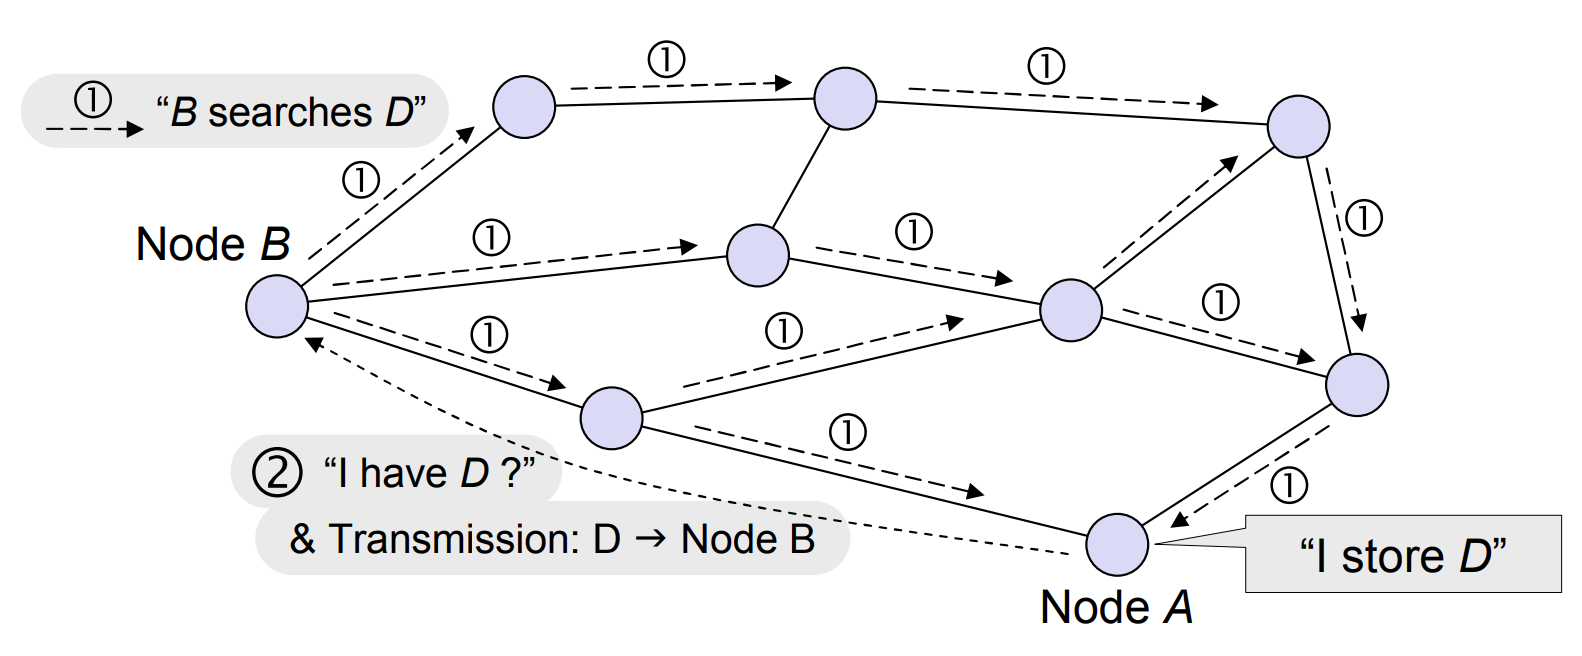
\includegraphics[width=0.7\textwidth]{images/02_flooding_search.png}
	\caption{\textbf{Flooding Search} : diffusion r\'ecursive de requ\^etes, puis retour des n\oe uds ayant la donn\'ee.}
	\label{fig:02_flooding_search}
\end{figure}

\newpage
\subsubsection*{3. Distributed Hash Tables (DHTs)}
Les DHTs (\emph{structured Peer-to-Peer systems}) structurent l'\emph{overlay} pour obtenir un compromis robuste : \(O(\log N)\) entr\'ees de routage par n\oe ud et \(O(\log N)\) \emph{hops} pour localiser une donn\'ee.

\begin{figure}[!ht]
	\centering
		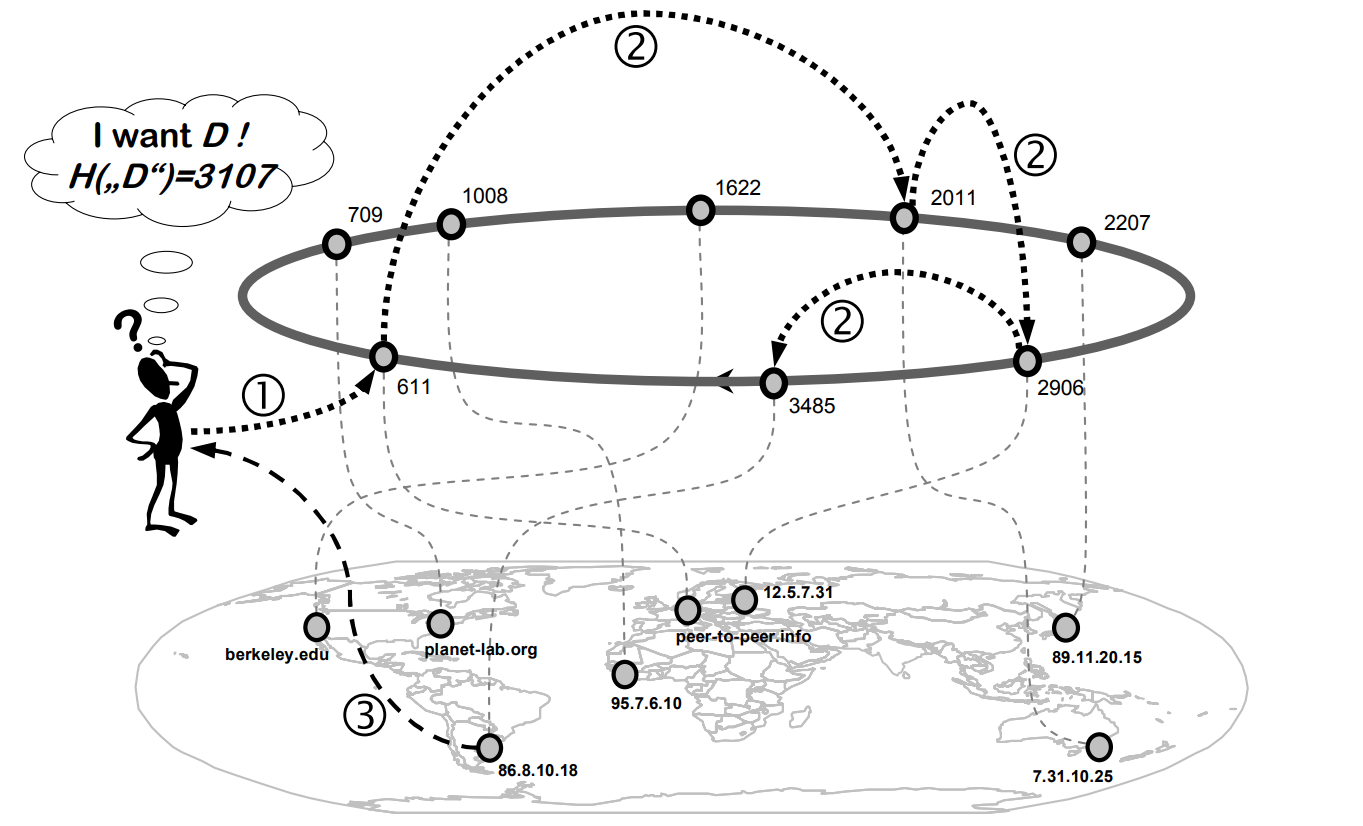
\includegraphics[width=0.7\textwidth]{images/04_dht_principle.png}
	\caption{\textbf{Distributed Hash Table} : routage structur\'e et efficace vers le n\oe ud responsable.}
	\label{fig:04_dht_principle}
\end{figure}

Les Figures~\ref{fig:01_central_server}, \ref{fig:02_flooding_search}, \ref{fig:04_dht_principle} et~\ref{fig:03_comparison_central_flooding_dht} montrent que les DHTs offrent le meilleur compromis entre co\^ut de recherche et co\^ut de stockage.

\begin{figure}[!ht]
	\centering
		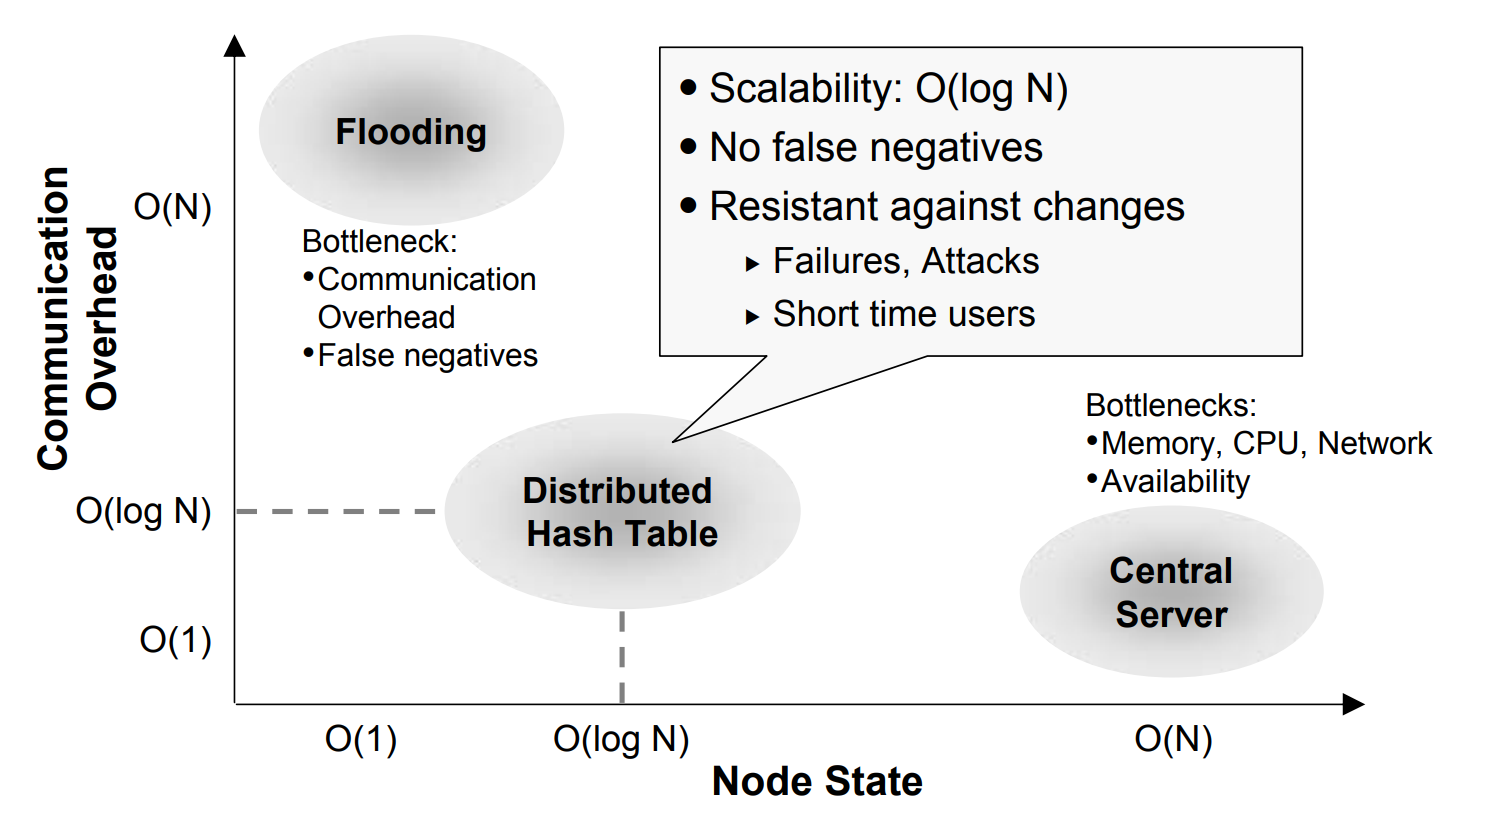
\includegraphics[width=0.7\textwidth]{images/03_comparison_central_flooding_dht.png}
\caption{Comparaison de la complexit\'e en termes d'effort de recherche (axe y) et de co\^ut de stockage par n\oe ud (axe x). Les goulots d'\'etranglement (\emph{bottlenecks}) ainsi que les caract\'eristiques sp\'ecifiques de chaque approche sont indiqu\'es.}
	\label{fig:03_comparison_central_flooding_dht}
\end{figure}

\newpage
\subsubsection{Fondamentaux des Distributed Hash Tables}

Une DHT associe chaque cl\'e \`a un n\oe ud responsable via un espace d'adressage logique et un routage d\'eterministe.

\subsubsection*{Gestion distribu\'ee des donn\'ees}
Chaque n\oe ud g\`ere une plage de cl\'es et conserve une \emph{partial view} du syst\`eme. Les messages sont relay\'es de n\oe ud en n\oe ud jusqu'\`a la destination.

\subsubsection*{Adressage dans les Distributed Hash Tables}
N\oe uds et donn\'ees partagent le m\^eme \emph{address space} logique (souvent tr\`es grand, p.~ex. \(0\) \`a \(2^{160}-1\)). Les IDs sont produits par une \emph{collision-resistant hash function}.

\begin{figure}[!ht]
	\centering
		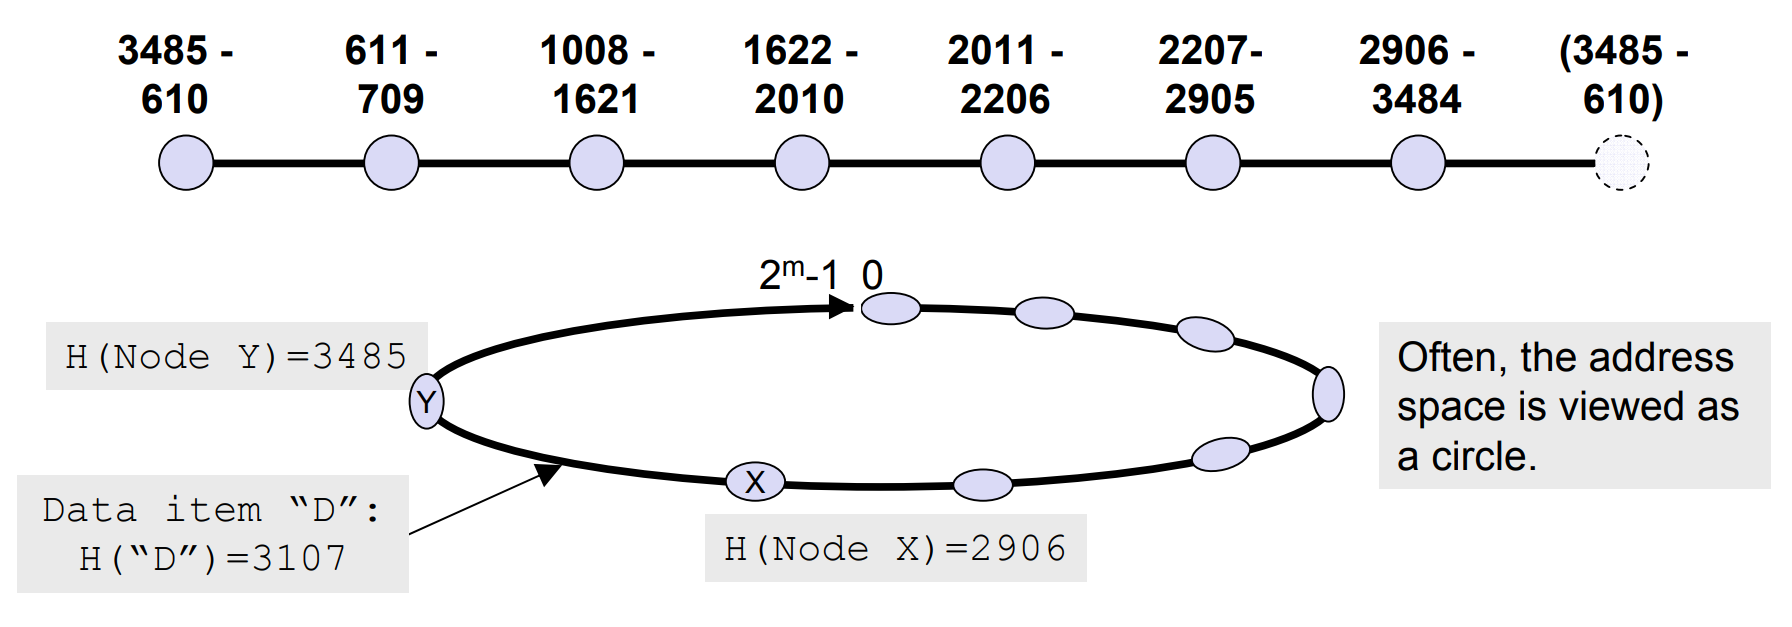
\includegraphics[width=0.7\textwidth]{images/05_a_linear_address_space_in_dht.png}
	\caption{Espace d'adressage lin\'eaire partitionn\'e entre pairs.}
	\label{fig:05_a_linear_address_space_in_dht}
\end{figure}

\begin{figure}[!ht]
	\centering
		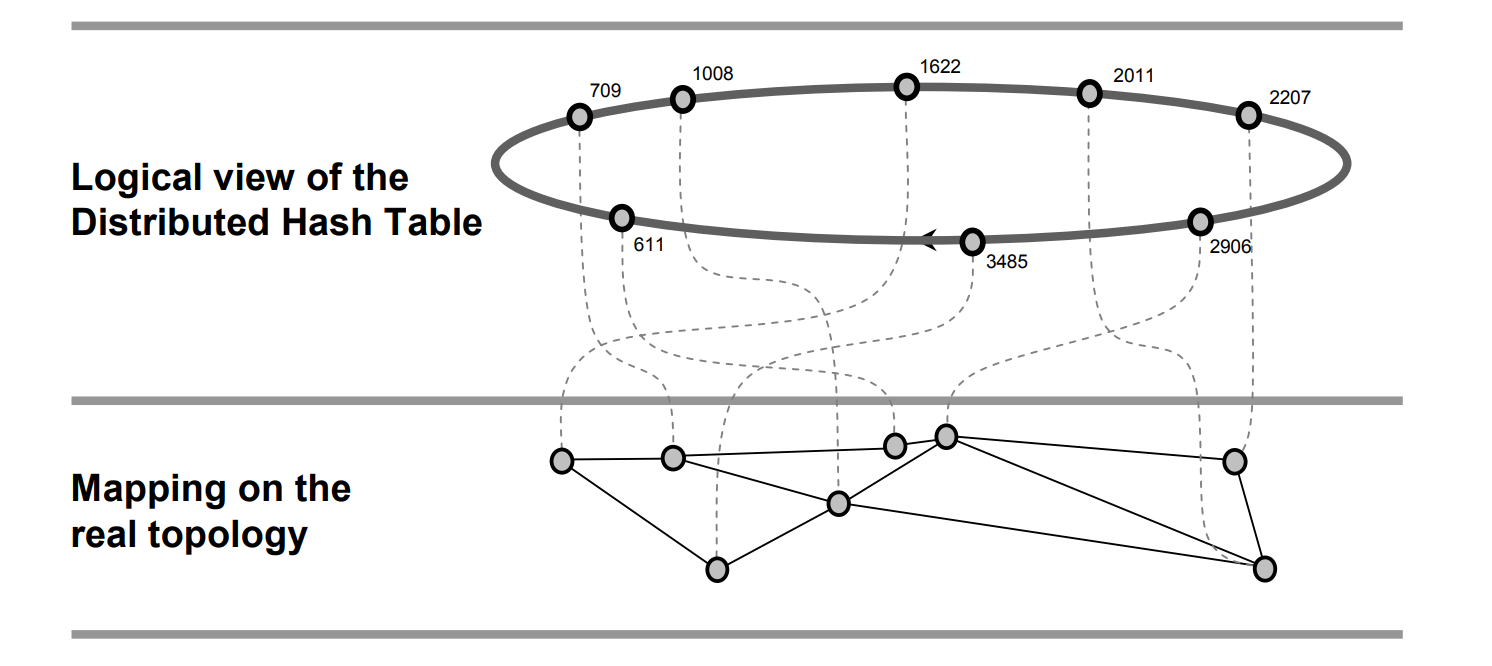
\includegraphics[width=0.7\textwidth]{images/06_underlay_view_of_dht.png}
	\caption{Vue logique de la DHT et vue du r\'eseau sous-jacent.}
	\label{fig:06_underlay_view_of_dht}
\end{figure}

\subsubsection*{Routage}
Chaque n\oe ud transmet vers un voisin plus proche de l'ID cible, ce qui r\'eduit progressivement la distance jusqu'au n\oe ud responsable en un \emph{small number of hops}.

\subsubsection*{M\'ethodes de stockage}
\textbf{Direct Storage} : la donn\'ee est copi\'ee sur le n\oe ud responsable (meilleure \emph{availability}, co\^ut plus \'elev\'e).

\textbf{Indirect Storage} : la DHT stocke un \emph{pointer} vers la donn\'ee (co\^ut r\'eduit, d\'ependance au n\oe ud source).

\begin{figure}[!ht]
	\centering
		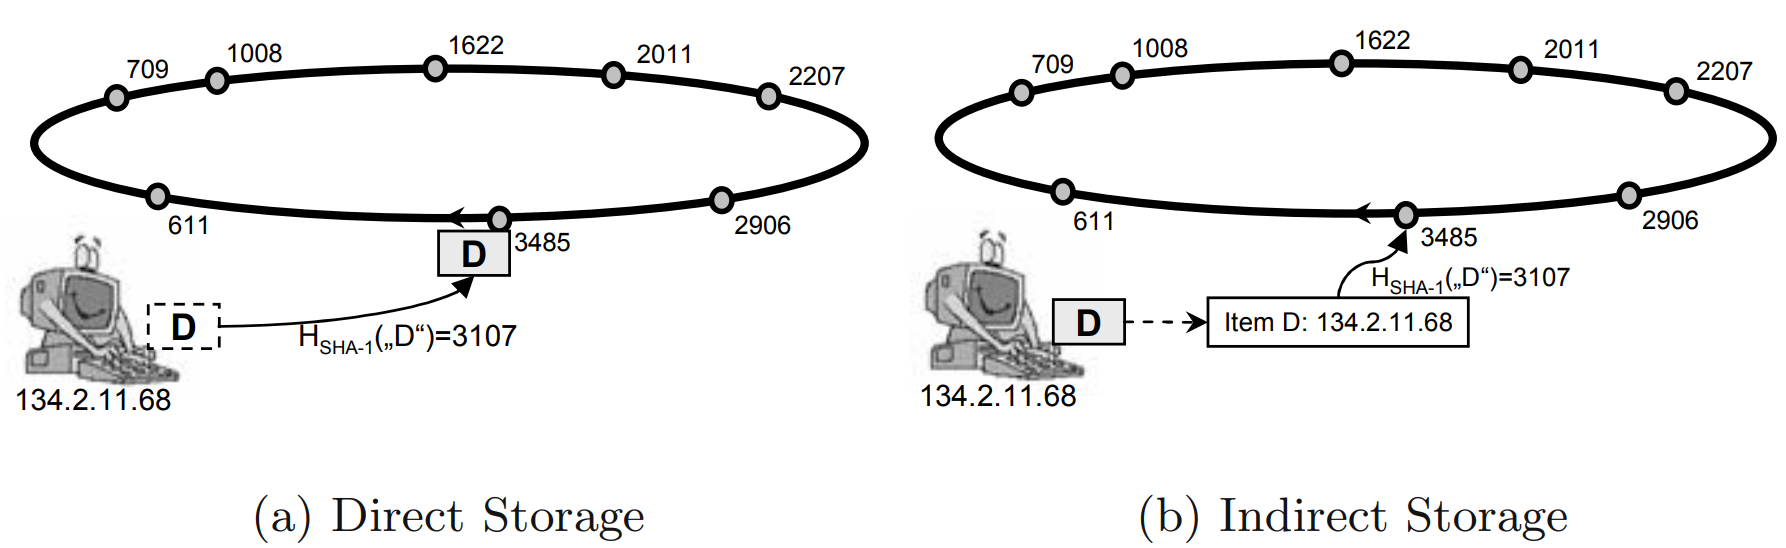
\includegraphics[width=0.7\textwidth]{images/07_direct_indirect_storage.png}
	\caption{Comparaison entre stockage direct et stockage indirect.}
	\label{fig:07_direct_indirect_storage}
\end{figure}

\subsubsection{M\'ecanismes des DHTs}

La robustesse d\'epend de la gestion du \emph{churn}, c'est-\`a-dire le taux de \emph{joins} et \emph{leaves} (arriv\'ees/d\'eparts) ainsi que les pannes fr\'equentes.

\subsubsection*{Arriv\'ee de n\oe uds}
L'entr\'ee d'un n\oe ud suit quatre \'etapes courtes :
\begin{enumerate}
\item \textbf{Bootstrap} : le nouveau pair contacte un n\oe ud existant qui sert d'\emph{entry point}.
\item \textbf{Address Assignment} : il re\c{c}oit sa partition dans le \emph{logical address space}.
\item \textbf{Routing Update} : les tables de routage sont ajust\'ees pour int\'egrer le nouveau pair.
\item \textbf{Data Transfer} : les paires \emph{(key, value)} devenues sa responsabilit\'e lui sont transf\'er\'ees.
\end{enumerate}

\subsubsection*{D\'efaillance de n\oe uds}
Deux approches coexistent : \emph{reactive recovery} (d\'etection pendant le routage, puis route alternative) et \emph{proactive recovery} (\emph{probes} p\'eriodiques, remplacement pr\'eventif des entr\'ees invalides). La \emph{replication} limite la perte de donn\'ees applicatives.

\subsubsection*{D\'epart de n\oe uds}
Un d\'epart volontaire (\emph{graceful leave}) facilite la migration imm\'ediate des donn\'ees vers le \emph{successor} et acc\'el\`ere la convergence des tables de routage. Il am\'eliore aussi la \emph{routing efficiency} et stabilise les m\'ecanismes de \emph{replication} et de \emph{load-balancing}.

\newpage
\subsubsection{Interfaces des DHTs}

\begin{figure}[h]
	\centering
		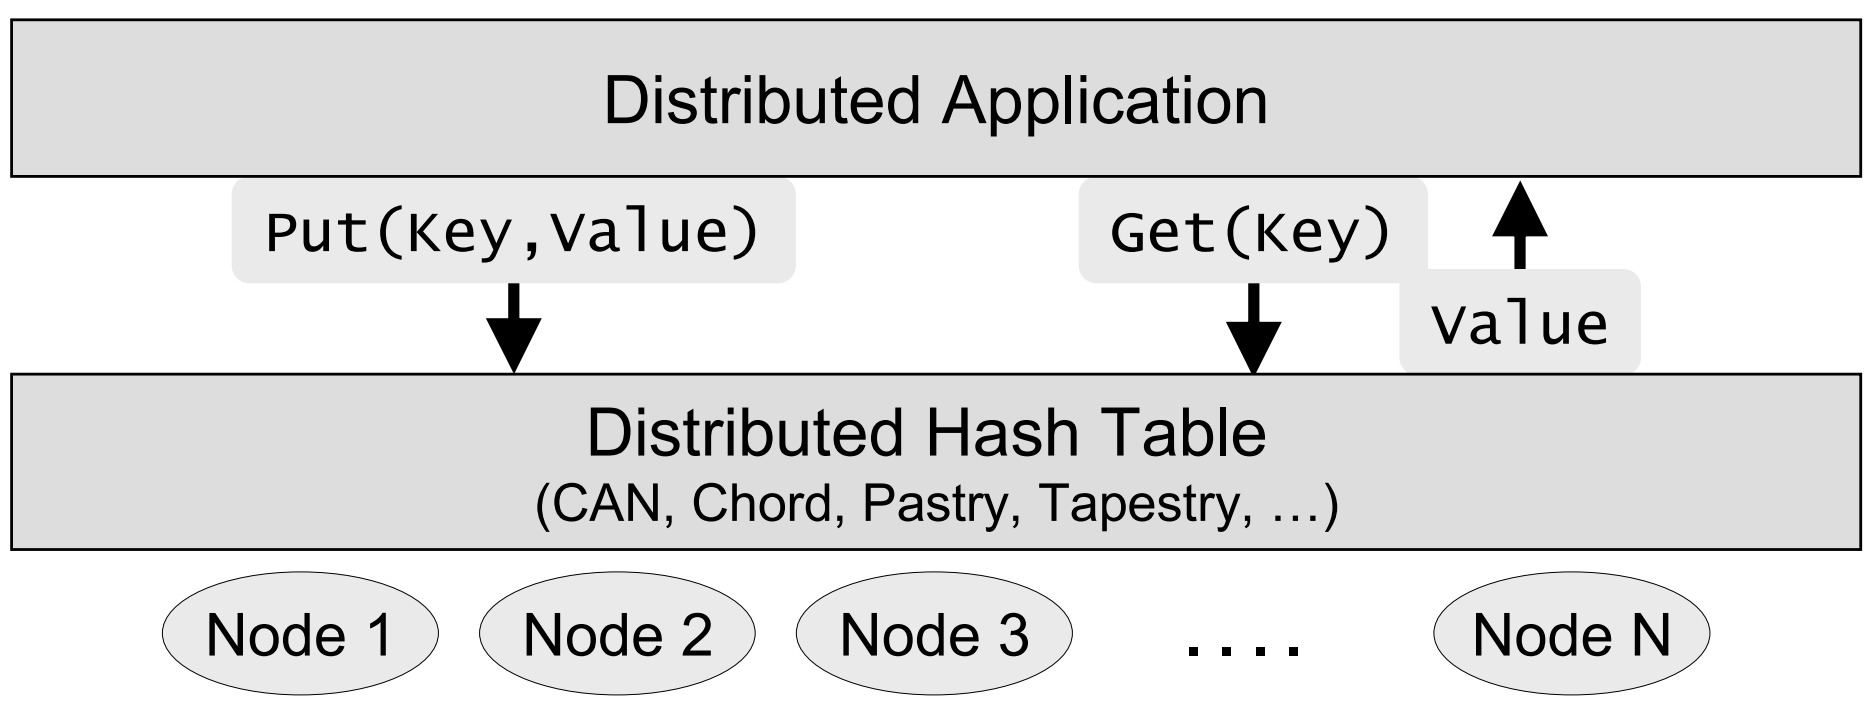
\includegraphics[width=0.5\textwidth]{images/08_interface_of_a_dht.png}
	\caption{Interface d'une Distributed Hash Table, typiquement \textsf{put}/\textsf{get}.}
	\label{fig:08_interface_of_a_dht}
\end{figure}

\subsubsection*{Interface de routage}
Interface \emph{stateless} orient\'ee messages : \texttt{send} livre vers un ID destination, \texttt{receive} remet les messages \`a l'application (\emph{delivery semantics}).
Cette \emph{stateless interface} se concentre sur la livraison de paquets bas\'es sur un ID logique plut\^ot que sur une adresse IP physique.

\subsubsection*{Interface de stockage}
Interface cl\'e-valeur : \texttt{put} \'ecrit la donn\'ee, \texttt{get} la r\'ecup\`ere. La couche g\`ere \emph{routing failures}, \emph{replication} et \emph{admission control}.
Cette couche ajoute de la complexit\'e car elle g\`ere la persistance et la fiabilit\'e des donn\'ees, comme une table de \emph{hash} distribu\'ee.

\subsubsection*{Interface Client}
Des h\^otes peuvent consommer le service DHT sans participer au routage de l'\emph{overlay} (mode \emph{client}).
Ce mode est utile quand on veut s\'eparer usage applicatif et participation au routage (fiabilit\'e, politiques d'\emph{access control}).

%\newpage
\subsubsection{Conclusions}

Les DHTs offrent une excellente \emph{scalability} sans point central, mais imposent des compromis entre efficacit\'e de routage, co\^ut de maintenance et r\'esilience au \emph{churn}.

\subsubsection*{D\'efis de conception}
\begin{itemize}
\item \textbf{Routing Efficiency} : qualit\'e du routage selon la structure des tables et la topologie.
\item \textbf{Management Overhead} : co\^ut de maintenance en continu.
\item \textbf{Churn} : impact des arriv\'ees/d\'eparts simultan\'es sur la stabilit\'e.
\end{itemize}

\subsubsection*{Limitations fondamentales}
\begin{itemize}
\item \textbf{Untrusted Environments} : r\'esistance difficile face aux n\oe uds malveillants et aux \emph{Byzantine faults}.
\item \textbf{Query Constraints} : \emph{fuzzy searches} et requ\^etes textuelles complexes peu adapt\'ees au mod\`ele par identifiants.
\end{itemize}

\newpage
\subsection{\'Etude de l'approche hi\'erarchis\'ee : HBase}

Les DHT repondent bien au \emph{lookup} en environnement dynamique, mais certaines applications exigent davantage de controle sur la coherence, la persistance et les performances de scan/ecriture. L'approche hi\'erarchis\'ee d'Apache HBase repond a ce besoin.

\subsubsection{Introduction au modele hierarchise}

HBase, construit sur HDFS (\emph{Hadoop Distributed File System}), est une base NoSQL distribu\'ee orient\'ee grands volumes. Contrairement aux DHT decentralisees, HBase suit un modele \emph{master-worker} avec \emph{range partitioning} : adressage d\'eterministe par \emph{row key}, scans sequentiels efficaces et coherence forte au niveau ligne.

\subsubsection{Fondamentaux architecturaux de HBase}

Le \emph{HBase Master} g\`ere le cluster (allocation des regions, equilibrage, d\'etection de pannes), tandis que les \emph{RegionServers} stockent les donn\'ees et executent les lectures/ecritures. Cette separation simplifie l'administration et le controle operationnel.

\subsubsection*{Mod\`ele de donn\'ees et espace d'adressage}

Le modele est oriente colonnes (tables, \emph{rows}, familles de colonnes). Les \emph{row keys} ordonnees lexicographiquement definissent l'espace d'adressage : excellent pour les scans et les requ\^etes par plages, mais sensible au design des cles.


\subsubsection{M\'ecanismes internes : partitionnement et gestion des pannes}

Deux mecanismes portent la scalabilite et la durabilite : partitionnement par regions et reaffectation apres panne.

\subsubsection*{Partitionnement horizontal par plages de cles}

Les tables sont decoupees en regions couvrant des plages continues de \emph{row keys}. Avec la croissance des donn\'ees, \emph{region splitting} repartit la charge entre RegionServers. Limite cl\'e : des cles monotones (ex.~timestamps) creent des \emph{hotspots} et du \emph{data skew} (\emph{storage skew}/\emph{access skew}).

Par rapport au \emph{consistent hashing} des DHT (distribution pseudo-aleatoire), HBase choisit un partitionnement d\'eterministe par ordre de cles.

\subsubsection*{Gestion des pannes et reaffectation}

En cas de panne d'un RegionServer, le Master (avec ZooKeeper) reassigne les regions. Avec le \emph{WAL} et HDFS, la reconstruction est robuste. Ce modele est centralise, contrairement a la reorganisation incrementale des DHT.


\subsubsection{Avantages et limites}

\textbf{Avantages.} Coherence forte en lecture/ecriture, tr\`es bonnes performances de scans sequentiels, et bonne scalabilite horizontale via \emph{region splitting} + ajout de RegionServers.

\textbf{Limites.} Forte sensibilite au schema de cles (risque de \emph{hotspot} et \emph{data skew}) et complexit\'e operationnelle elevee (HDFS, ZooKeeper, tuning et supervision du cluster).

\subsection{Conclusion et justification du choix architectural}

DHT et HBase repondent au meme objectif (stockage distribue a grande echelle) avec des choix opposes : decentralisation + \emph{consistent hashing} d'un cote, coordination centralisee + \emph{range partitioning} de l'autre.

\subsubsection*{Crit\`ere d'\'evaluation : gestion du data skew}

Le \emph{data skew} est determinant : HBase peut concentrer charge/stockage si les cles sont mal concues, alors que les DHT reduisent structurellement ce risque via une distribution pseudo-aleatoire des identifiants.

\subsubsection*{Motivation du choix}

Notre objectif est d'implementer un systeme totalement decentralise en anneau logique. Les DHT sont mieux alignees avec cet objectif (routage distribue, auto-organisation, joins/leaves, absence de maitre), tandis qu'une approche HBase deplacerait le projet vers l'ingenierie d'un cluster hierarchise.

\subsubsection*{Conclusion du choix}

HBase reste excellent pour des besoins de coherence forte et de scans massifs, mais pour nos objectifs pedagogiques/experimentaux, l'approche DHT est plus pertinente.
En consequence, nous retenons l'architecture DHT comme base de la suite du projet.


\section{Méthode de répartition des données}

\subsection{Motivation et définition de la répartition des données}

Avec l’augmentation continue du volume de données et du nombre d’utilisateurs, les architectures de stockage centralisées atteignent rapidement leurs limites. Une base de données unique n’a plus la capacité de contenir toute ces données et constitue un point de défaillance susceptible de compromettre la disponibilité du système.

\IfFileExists{images/09_central_architecture.png}{
\begin{figure}[!ht]
\centering
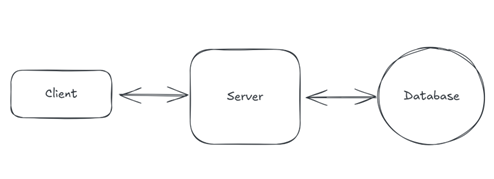
\includegraphics[width=0.7\textwidth]{images/09_central_architecture.png}
\end{figure}
}{}

Une solution pour pallier à ces limitations consiste à répartir les données et les requêtes sur plusieurs bases de données, afin de distribuer la charge de stockage et de traitement, et d’éviter la surcharge d’une base de données unique.

\newpage

\IfFileExists{images/10_distributed_architecture.png}{
\begin{figure}[!ht]
\centering
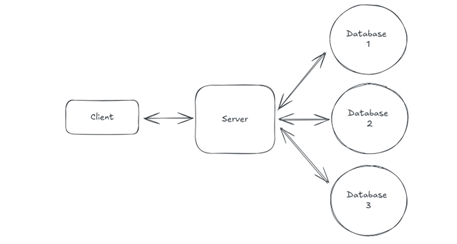
\includegraphics[width=0.7\textwidth]{images/10_distributed_architecture.png}
\end{figure}
}{}

Toutefois, cette distribution soulève un problème fondamental : il devient nécessaire de déterminer de manière systématique sur quelle base de données une donnée doit être stockée et comment la retrouver efficacement. C’est pour répondre à cette problématique que les méthodes de répartition des données (data partitioning ou data sharding) ont été introduites. Elles définissent les règles de placement des données ce qui impacte directement les performances et l’équilibrage de charge. Ces méthodes de répartitions des données impactent également l’évolution du système dans le temps, c’est-à-dire lors de l’ajout ou le retrait d’une base de données.

\subsection{Les différentes méthodes de répartitions des données}

Après avoir montré la nécessité de répartir les données dans un système distribué, la première question qu’on se pose : comment associer chaque donnée à une base de données ?

Différentes méthodes de répartition des données permettent d’associer une clé à une base de données dans un système distribué.

Dans les exemples suivant nous allons utiliser le termes nœud qui fait référence à une instance base de données et le terme évènement qui fait référence à une donnée.

\subsubsection{hachage classique}

\subsubsection*{Principe général du hachage classique}

Une première approche naïve appelée hachage classique (naive hashing ou modulo hashing) consiste à utiliser une fonction de hachage afin de faire la correspondance entre la clé d’une donnée et la base de données dans laquelle nous allons la stocker.

\newpage
\subsubsection*{Association d’une clé à un nœud}

Cette méthode repose sur les étapes suivantes :



\begin{enumerate}
\item Prendre l’id de l’événement et l’exécuter via une fonction de hachage, qui le convertit en nombre
\item Prendre ce nombre et effectuer l’opération modulo (\%) avec le nombre de base de données.
\item Le résultat nous indique quelle base de données doit stocker cet évènement.
\end{enumerate}

La formule serait donc :

\[
\texttt{database\_id} = \texttt{hash(event\_id)} \bmod \texttt{number\_of\_databases}
\]

\IfFileExists{images/11_hash_modulo.png}{
\begin{figure}[!ht]
\centering
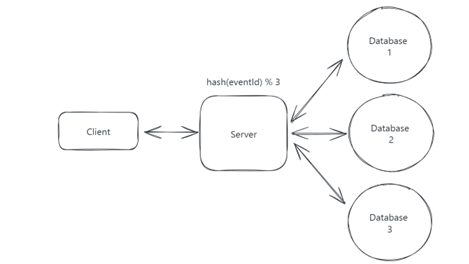
\includegraphics[width=0.6\textwidth]{images/11_hash_modulo.png}
\end{figure}
}{}

Pour un exemple concret avec 3 bases de données :

Event \#1234 → hash(1234) \% 3 = 1 → Database 2

Event \#5678 → hash(5678) \% 3 = 0 → Database 1

Event \#9012 → hash(9012) \% 3 = 2 → Database 3

Ainsi, chaque clé est associée à une base de données unique, ce qui permet de retrouver l’emplacement d’une donnée à partir de sa clé.

\subsubsection*{Limite du hachage classique}

Le premier problème survient lorsque l’on souhaite ajouter une nouvelle instance de base de données. La première solution à laquelle on pourrait penser consisterait à exécuter l'opération modulo avec 4 au lieu de 3 (Par rapport à l’exemple précédent).


database\_id = hash(event\_id) \% 4


La modification du nombre total de bases de données a non seulement affecté les données destinées à la nouvelle instance, mais a également entraîné une modification de la base de données associé à chaque événement précédemment stocké.

En effet, si on reprend un des exemples précédents :

Event \#1234 → hash(1234) \% 3 = 1 → Database 2     hash(1234) \% 4 = 0 → Database 1

L'événement n° 1234 était mappé à la base de données 2, mais avec l’ajout de la nouvelle base de données, ces données doivent donc être déplacées vers la base de données 1.

\newpage
\IfFileExists{images/12_hash_resize_problem.png}{
\begin{figure}[!ht]
\centering
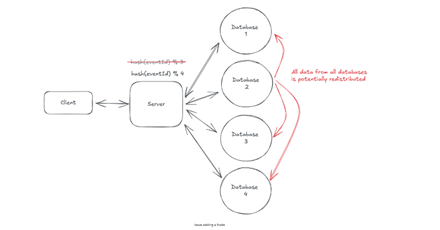
\includegraphics[width=0.7\textwidth]{images/12_hash_resize_problem.png}
\end{figure}
}{}

L’ajout d’une ou plusieurs bases de données entraîne donc une redistribution dans toutes les instances de base de données, ce qui provoque un mouvement massif de données inutiles. Ce mouvement massif cause d'énormes pics de charge de base de données et impact directement les utilisateurs. En effet, les utilisateurs ne pourront pas accéder à leur donner ou auront un temps de réponse lent.


Un autre problème avec le hachage modulo simple réside dans le retrait d’une base de données. Supposons qu'une base de données soit tombée en panne. Il est nécessaire de redistribuer les données qui étaient dans la base de données tombé en panne vers les autres bases de données encore actives. Etant donné que le nombre de base de données actives diminue, le calcule pour trouver où ranger une donnée sera modifié. De ce fait, les données présentes dans les bases de données encore actives risque d’être redistribué vers d’autre instance de base de données.

\IfFileExists{images/13_hash_resize_problem2.png}{
\begin{figure}[!ht]
\centering
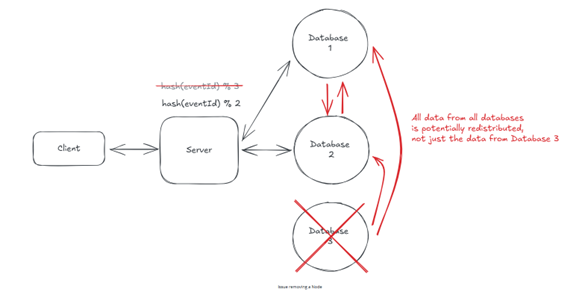
\includegraphics[width=0.7\textwidth]{images/13_hash_resize_problem2.png}
\end{figure}
}{}

Ces limitations montrent que le hachage modulo classique n’est pas adapté aux systèmes distribués dynamiques, où les bases de données peuvent être ajoutés ou retirés fréquemment.

\subsubsection{Hachage cohérent (Consistent Hashing)}

\subsubsection*{Principe général du consistent Hashing}

Le consistent Hashing a été introduit pour résoudre le problème de la redistribution des données lors de l'ajout ou de la suppression d'une instance dans un système distribué. Le principe est d’organiser à la fois les données et les bases de données dans un espace circulaire appelé « anneau de hachage ».

Dans cet anneau, les clés et les nœuds sont positionnés en utilisant la même fonction de hachage. Chaque base de données se voit attribuer une position sur l’anneau, et chaque donnée est également positionnée sur cet anneau en fonction du résultat de sa fonction de hachage.


\subsubsection*{Association d’une clé à un nœud}

Cette méthode repose sur les étapes suivantes :

\begin{enumerate}
\item On réalise d’abord un anneau de hachage avec un nombre fixe de points.
\item On positionne les bases de données sur l’anneau en appliquant la fonction de hachage à leur identifiant.
\item Pour trouver sur quelle base de données une donnée doit être stockée, on hache d'abord l'ID de la donnée comme avec le hachage classique.
\item On se déplace ensuite dans le sens des aiguilles d'une montre sur l’anneau jusqu’à rencontrer le premier nœud.
\item Ce nœud va stocker de la donnée.
\end{enumerate}

Par exemple :

Pour un nombre fixe de points égal à 90, 3 bases de données positionnées aux points 20, 50 et 80.

Si nous avons un $\texttt{hash(id\_data)} = 32$, nous nous déplaçons dans le sens des aiguilles d’une montre pour trouver la première instance de base de données. Cette instance sera la base de données 2 (Node B) située au point 50.

\IfFileExists{images/14_consistent_example.png}{
\begin{figure}[!ht]
\centering
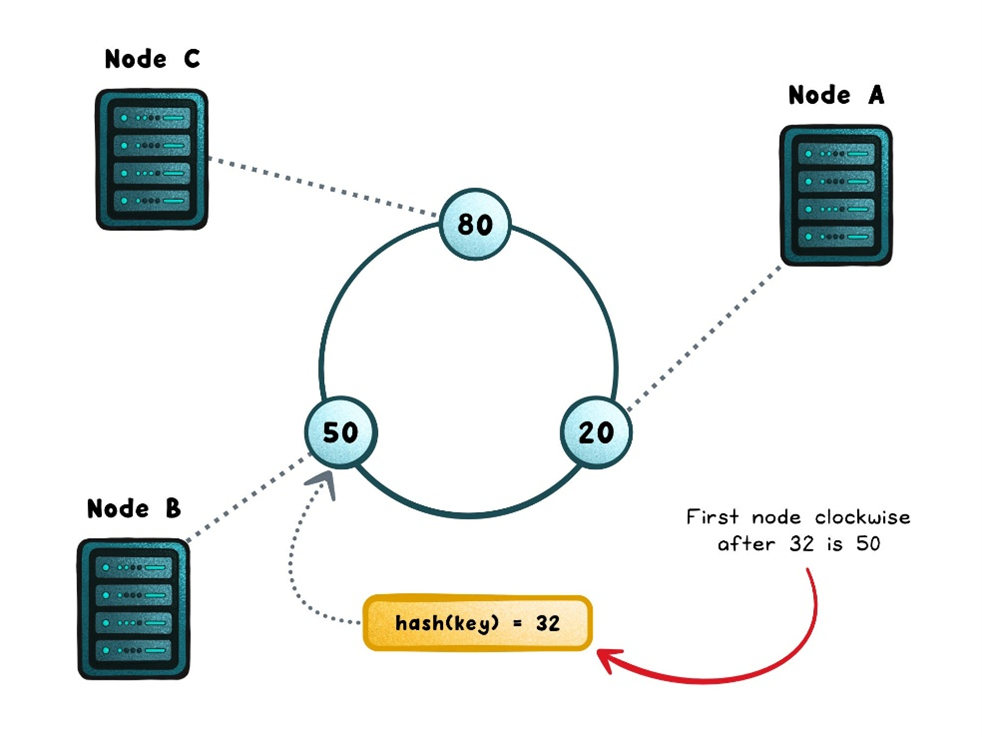
\includegraphics[width=0.75\textwidth]{images/14_consistent_example.png}
\end{figure}
}{}

\subsubsection*{Ajout d’une nouvelle base de données}

Lorsqu’on ajoute une nouvelle base de données, seules les données qui se situent entre sa nouvelle position et la base de données précédente doivent être déplacées.

Par exemple :

Pour un nombre fixe de points égal à 100, 4 bases de données positionnées aux points 0, 25, 50 et 75.

Si nous ajoutons une cinquième base de données à la position 90 sur notre anneau :

\begin{itemize}
	\item Seules les données qui se hachent vers des positions comprises entre 75 et 90 doivent désormais être stockées dans la base de données 5.

  \item Toutes les autres données restent dans leur base de données respective.
\end{itemize}

\IfFileExists{images/15_consistent_add.png}{
\begin{figure}[!ht]
\centering
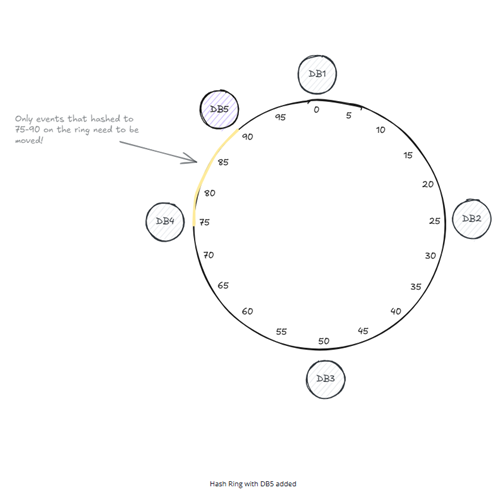
\includegraphics[width=0.75\textwidth]{images/15_consistent_add.png}
\end{figure}
}{}

Contrairement au hachage modulo classique, seule une petite portion des données est redistribuée.

\subsubsection*{Suppression d’une base de données}

En reprenant l’exemple initial :

Pour un nombre fixe de points égal à 100, 4 bases de données positionnées aux points 0, 25, 50 et 75.

Supposons que la base de données numéro 2 située à la position 25 rencontre une défaillance.
\begin{itemize}
  \item Seules les données mappées sur la base de données 2 doivent être déplacées.

  \item Le déplacement se fait dans le sens des aiguilles d’une montre. Elles seront donc mappées à la base de données 3 située à la position 50.

	\item Toutes les autres données restent dans leur base de données respective.
\end{itemize}

\newpage

\IfFileExists{images/16_consistent_remove.png}{
\begin{figure}[!ht]
\centering
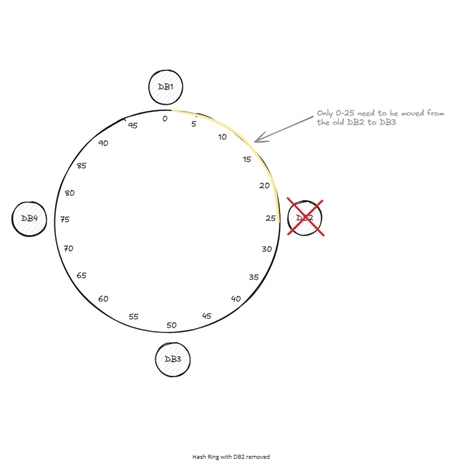
\includegraphics[width=0.75\textwidth]{images/16_consistent_remove.png}
\end{figure}
}{}

Le consistent hashing permet ainsi de résoudre les principales limites du hachage classique en réduisant drastiquement le nombre de données redistribuées lors des changements de topologie (ajout ou retrait de base de données). 

Cependant, il reste encore un problème. En effet, dans notre exemple ci-dessus où nous avons supprimé la base de données 2, nous avons dû déplacer toutes les données stockées dans la base de données 2 vers la base de données 3, ce qui peut entraîner une surcharge locale. Notre objectif serait de répartir de manière équitable les données lors de la suppression d’une base de données.  


\subsubsection*{Optimisation : Nœuds Virtuels}

Pour résoudre ce problème, une des solutions serait d’utiliser des « nœuds virtuels ». Au lieu de mettre chaque base de données en un seul point de sur l’anneau, nous la divisons en plusieurs point en hachant différentes variantes du nom de la base de données. 

Par exemple : 

« DB1 » sera diviser en « DB1-vn1 », « DB1-vn2 », « DB1-vn3 » et « DB1-vn4 » qui seront respectivement aux positions 0, 20, 35, 65, 80. C’est le même principe pour les autres bases de données.

\newpage

\IfFileExists{images/17_virtual_nodes.png}{
\begin{figure}[!ht]
\centering
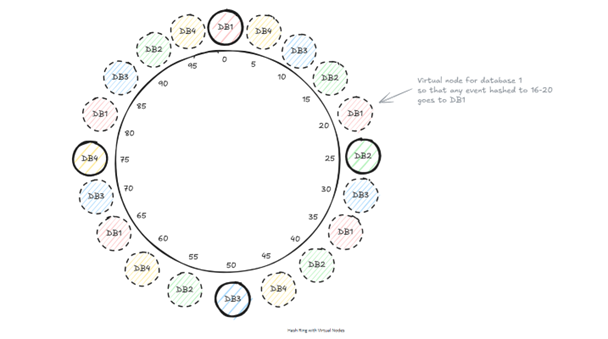
\includegraphics[width=0.8\textwidth]{images/17_virtual_nodes.png}
\end{figure}
}{}

Nous pouvons observer sur la figure ci-dessus que les nœuds virtuelles sont mélangés autour de l’anneau. 
Supposons que la bases de données numéro 2 rencontre une défaillance : 
	
	\begin{itemize}
		\item Les données mappées sur « DB2-vn1 » seront stockées dans la base de données 1
		\item Les données mappées sur « DB2-vn2 » seront stockées dans la base de données 3
    \item Les données mappées sur « DB2-vn3 » seront stockées dans la base de données 4
	  \item Et ainsi de suite
\end{itemize}
La charge de la base de données supprimé est donc répartie de manière beaucoup plus homogène dans toute les bases de données actives. 


\subsection{Conclusion sur les méthodes de répartitions des données}

Les méthodes de répartition des données sont donc indispensables dans les systèmes distribués. En effet, elles déterminent la manière dont les données sont réparties entre les bases de données. Le hachage classique est une solution simple, mais peu adaptée lors de l’ajout ou du retrait d’une ou plusieurs bases de données, en raison des redistributions massives qu’il engendre. Le consistent hashing permet de corriger ces limitations en réduisant les déplacements de données. Une des optimisations du consistent hashing repose sur l’utilisation de nœuds virtuels, permettant d’améliorer l’équilibrage de charge entre les nœuds lors du retrait d’une base de données.


\section{Chord}

Chord est un protocole DHT (\emph{Distributed Hash Table}) qui r\'esout un probl\`eme unique : trouver rapidement le n\oe ud responsable d'une cl\'e dans un r\'eseau pair-\`a-pair dynamique.

\subsection{Principe de fonctionnement}

Chaque n\oe ud et chaque cl\'e re\c coivent un identifiant sur \(m\) bits (souvent via SHA-1), plac\'e sur un anneau modulo \(2^m\). Une cl\'e \(k\) est stock\'ee sur son \emph{successor} : le premier n\oe ud rencontr\'e dans le sens horaire dont l'identifiant est sup\'erieur ou \`a \(k\).

Cette r\`egle donne trois propri\'et\'es utiles :
\begin{itemize}
\item \textbf{R\'epartition} : le \emph{consistent hashing} distribue les cl\'es de mani\`ere quasi uniforme.
\item \textbf{Scalabilit\'e} : l'ajout/retrait d'un n\oe ud ne d\'eplace qu'une fraction des cl\'es.
\item \textbf{D\'ecentralisation} : aucun serveur central n'est requis.
\end{itemize}

\subsection{Routage efficace : Finger Table}

Pour \`eviter un parcours lin\'eaire de l'anneau, chaque n\oe ud maintient une \textbf{finger table} de \(m\) entr\'ees. L'entr\'ee \(i\) pointe vers le premier n\oe ud joignable \`a partir de \(n + 2^{i-1}\).

\[
\text{finger}[i].\text{start} = (n + 2^{i-1}) \bmod 2^m
\]

Cette structure permet des sauts exponentiels et un co\^ut moyen de recherche en \(O(\log N)\) messages.

\subsection{Algorithmes essentiels}

\textbf{1) Recherche de la cl\'e : \texttt{find\_successor(id)}}
\begin{itemize}
\item Si \texttt{id} est entre le n\oe ud courant et son \emph{successor}, on retourne ce \emph{successor}.
\item Sinon, on avance vers le \emph{closest\_preceding\_node(id)} dans la finger table et on r\'ep\`ete.
\end{itemize}

\textbf{2) Choix du prochain saut : \texttt{closest\_preceding\_node(id)}}
\begin{itemize}
\item Parcours de la finger table du plus grand saut au plus petit.
\item Retour du premier doigt situ\'e strictement avant \texttt{id} sur l'anneau.
\end{itemize}

\textbf{3) Arriv\'ee d'un n\oe ud : \texttt{join(n')}}
\begin{itemize}
\item Le nouveau n\oe ud contacte un n\oe ud connu \(n'\).
\item Il initialise son \emph{successor} via \texttt{find\_successor} puis construit sa finger table.
\end{itemize}

\textbf{4) Stabilisation : \texttt{stabilize()} et \texttt{notify()}}
\begin{itemize}
\item Ex\'ecution p\'eriodique pour corriger les pointeurs \emph{successor}/\emph{predecessor}.
\item Garantit la convergence vers un anneau coh\'erent apr\`es churn mod\'er\'e.
\end{itemize}

\textbf{5) Tol\'erance aux pannes : \texttt{successor list}}
\begin{itemize}
\item Chaque n\oe ud conserve plusieurs successeurs de secours.
\item En cas de panne du successeur principal, le routage continue via le suivant vivant.
\end{itemize}

\subsection{Complexit\'e (r\'esum\'e)}
\begin{itemize}
\item \textbf{Lookup} : \(O(\log N)\) messages.
\item \textbf{Maintenance d'un join/leave} : surco\^ut logarithmique (d\'epend de la politique de mise \`a jour).
\item \textbf{M\'emoire par n\oe ud} : \(O(\log N)\) entr\'ees de routage.
\end{itemize}

En pratique, Chord fournit une base simple et robuste pour le \emph{lookup} distribu\'e : routage logarithmique, maintenance locale p\'eriodique et bonne r\'esilience aux variations du r\'eseau.

\section{Pastry}

Pastry est une infrastructure distribuée de localisation d’objets et de routage destinée aux systèmes pair-à-pair (P2P) à grande échelle. Elle repose sur une table de hachage distribuée (DHT), comparable à Chord, et fonctionne au-dessus d’Internet via un réseau overlay. Les nœuds logiques de Pastry ne correspondent pas nécessairement à la topologie physique du réseau IP, mais forment une structure virtuelle organisée selon l’espace des identifiants.

L’objectif fondamental de Pastry est d’acheminer efficacement un message associé à une clé donnée vers le nœud dont l’identifiant est numériquement le plus proche de cette clé. À l’instar de Chord, Pastry résout le problème du \textit{key-based routing}, mais adopte une approche différente fondée sur un routage par préfixes plutôt que sur une structure strictement circulaire.

\subsection{Architecture générale}

La conception de Pastry repose sur plusieurs principes structurants :

\subsubsection*{1. Décentralisation}
Aucun nœud ne possède de rôle central. Chaque participant maintient localement ses structures de routage, ce qui supprime tout point unique de défaillance.

\subsubsection*{2. Scalabilité logarithmique}
Le routage s’effectue en $O(\log N)$ sauts en moyenne, où $N$ est le nombre de nœuds du système, ce qui garantit le passage à grande échelle.

\subsubsection*{3. Auto-organisation}
Le protocole s’adapte dynamiquement aux arrivées et aux départs de nœuds (\textit{churn}) par la mise à jour progressive des structures de routage.

\subsubsection*{4. Localité réseau}
Lorsque plusieurs nœuds satisfont une contrainte de routage, Pastry privilégie celui qui est le plus proche selon une métrique réseau, réduisant ainsi la latence réelle des communications.

\subsection{Identifiants et espace de clés}

Chaque nœud Pastry possède un identifiant unique, appelé \textit{nodeId}, généralement codé sur 128 bits et dérivé d’une fonction de hachage cryptographique. De même, chaque message ou clé à router reçoit un identifiant correspondant dans le même espace.

L’espace d’identifiants est organisé en base $2^{b}$, où $b$ est un paramètre de configuration influençant la taille des tables de routage. Le routage s’effectue en recherchant le nœud actif dont le \textit{nodeId} est numériquement le plus proche de l’identifiant cible.

Contrairement à Chord, qui dispose d’un anneau strictement circulaire, Pastry utilise un routage par préfixes, où la distance est mesurée par la longueur du préfixe commun entre identifiants.

\subsection{Structures de routage}

Chaque nœud Pastry maintient trois structures principales : la \textit{Routing Table}, le \textit{Leaf Set} et le \textit{Neighbor Set}.

\subsubsection{1. Routing Table}

Organisée par préfixes d’identifiants, elle contient des pointeurs vers des nœuds partageant des préfixes communs avec le \textit{nodeId} courant. Cette structure permet de faire des sauts logarithmiques vers la destination, rapprochant le message à chaque étape.

Cette structure est analogue aux \textit{Finger Tables} de Chord, mais basée sur des préfixes plutôt que sur des puissances de 2.

\subsubsection{2. Leaf Set (ensemble des feuilles)}

Il regroupe les nœuds immédiatement supérieurs et inférieurs au \textit{nodeId}. Il assure le routage correct pour les clés proches et fournit des alternatives en cas de défaillance de certains nœuds.

\subsubsection{3. Neighbor Set (ensemble des voisins)}

Il contient des nœuds physiquement proches selon la topologie réseau, indépendamment des identifiants. Il est utilisé pour optimiser la latence des communications et améliorer la localité réelle du routage.

\subsection{Processus de routage}

Le routage dans Pastry s’effectue en rapprochant progressivement le message de son \textit{nodeId} cible grâce aux structures précédentes :

\begin{enumerate}
    \item \textbf{Vérification du Leaf Set} : si la clé cible se trouve dans l’intervalle couvert, le message est envoyé au nœud le plus proche numériquement.
    \item \textbf{Utilisation de la Routing Table} : si la clé n’est pas dans le Leaf Set, le message est transmis à un nœud partageant un préfixe plus long avec la clé.
    \item \textbf{Sélection par proximité physique} : si aucune entrée n’est disponible ou valide, un nœud du Leaf Set numériquement plus proche est choisi, en prenant en compte la distance réseau.
\end{enumerate}

À chaque étape, le message progresse vers un nœud plus proche de la destination, ce qui garantit la convergence du routage en $O(\log N)$ sauts en moyenne pour $N$ nœuds actifs.

\subsection{Algorithmes des nœuds et maintenance}

Chaque nœud Pastry exécute des algorithmes pour intégrer de nouveaux nœuds, maintenir les structures de routage et gérer les défaillances.

\begin{enumerate}
    \item \textbf{Intégration d’un nouveau nœud (\textit{join})}
    \begin{itemize}
        \item Un nœud entrant contacte un nœud existant pour s’intégrer au réseau.
        \item Les structures de routage (\textit{Routing Table}, \textit{Leaf Set}, \textit{Neighbor Set}) sont initialisées progressivement grâce aux informations des nœuds voisins.
    \end{itemize}

    \item \textbf{Maintenance dynamique (\textit{stabilize} et mise à jour du routage)}
    \begin{itemize}
        \item Les entrées de la \textit{Routing Table} sont périodiquement mises à jour pour refléter les départs ou arrivées de nœuds.
        \item Le \textit{Leaf Set} et le \textit{Neighbor Set} sont également ajustés pour maintenir la cohérence et la résilience locale.
    \end{itemize}

    \item \textbf{Tolérance aux pannes}
    \begin{itemize}
        \item En cas de défaillance d’un nœud, les messages sont redirigés vers le nœud le plus proche dans le \textit{Leaf Set} ou via la \textit{Routing Table}.
        \item Cette redondance garantit que le routage reste correct et efficace même avec un nombre important de nœuds défaillants.
    \end{itemize}
\end{enumerate}


\section{Architecture du syst\`eme et cycle de vie d'une requ\^ete}

\subsection{Choix architecturaux et probl\'ematique}

Dans le cadre de notre projet, nous avons choisi d'impl\'ementer une architecture de stockage distribu\'ee reposant sur des protocoles de type Distributed Hash Table (DHT), et plus pr\'ecis\'ement sur Chord et Pastry. Ces deux protocoles partagent un objectif commun : organiser un ensemble de n\oe uds distribu\'es de mani\`ere totalement d\'ecentralis\'ee afin d'assurer le stockage et la localisation efficace de donn\'ees dans un espace d'identifiants partag\'e.

Avant d'impl\'ementer ces protocoles, il est essentiel de comprendre pr\'ecis\'ement l'architecture que nous allons construire ainsi que le protocole applicatif qui s'appuiera dessus. Autrement dit, nous devons \^etre capables de r\'epondre aux questions suivantes :

\begin{itemize}
    \item \`A quel n\oe ud une requ\^ete est-elle envoy\'ee initialement ?
    \item Comment est d\'etermin\'e le n\oe ud responsable d'une donn\'ee ?
    \item Comment les n\oe uds communiquent-ils entre eux ?
    \item Que se passe-t-il concr\`etement lors d'une op\'eration \'el\'ementaire telle que PUT ou GET ?
    \item Quel est le cycle de vie complet d'une requ\^ete ?
\end{itemize}

Dans cette premi\`ere partie, nous d\'etaillons l'architecture retenue pour Chord, en analysant pr\'ecis\'ement la circulation des messages, la responsabilit\'e des n\oe uds et le traitement des requ\^etes. La m\^eme d\'emarche sera ensuite appliqu\'ee \`a Pastry.

\subsubsection{Architecture g\'en\'erale bas\'ee sur Chord}

R\'esumons l'architecture Chord vue pr\'ec\'edemment en indiquant les diff\'erentes variables qui nous seront indispensables lors de son impl\'ementation. L'architecture Chord repose sur un espace d'identifiants circulaire de taille $2^m$. Cet espace est partag\'e \`a la fois par les n\oe uds du syst\`eme et par les cl\'es des donn\'ees stock\'ees. Chaque n\oe ud re\c coit un identifiant unique calcul\'e via une fonction de hachage, et se positionne sur un anneau logique selon cet identifiant.

Le principe fondamental de Chord est le suivant : une cl\'e est stock\'ee sur le premier n\oe ud dont l'identifiant est sup\'erieur ou \'egal \`a l'identifiant de la cl\'e dans le sens des aiguilles d'une montre. Ce n\oe ud est appel\'e le successeur de la cl\'e. Cette r\`egle garantit un placement d\'eterministe et uniforme des donn\'ees sans coordination centrale.

Chaque n\oe ud maintient localement plusieurs structures essentielles :

\begin{itemize}
    \item son identifiant unique,
    \item un pointeur vers son successeur,
    \item un pointeur vers son pr\'ed\'ecesseur,
    \item une table de routage appel\'ee finger table,
    \item un stockage local des paires (cl\'e, valeur).
\end{itemize}

La finger table permet d'assurer un routage logarithmique. Chaque entr\'ee de cette table pointe vers un n\oe ud situ\'e exponentiellement plus loin sur l'anneau. Ainsi, lorsqu'un n\oe ud doit localiser le responsable d'une cl\'e, il peut se rapprocher de la destination en un nombre de sauts proportionnel \`a $O(\log N)$, o\`u $N$ est le nombre total de n\oe uds.

\subsubsection{Couche Overlay et Couche applicative}

Il est essentiel, dans notre impl\'ementation, de distinguer clairement deux niveaux fonctionnels qui coexistent au sein de chaque n\oe ud.

Le premier niveau correspond \`a la couche overlay, c'est-\`a-dire le protocole Chord lui-m\^eme. Cette couche est responsable de l'organisation logique du r\'eseau en anneau, du maintien des pointeurs (successeur, pr\'ed\'ecesseur, finger table) et du routage des messages. Son r\^ole est exclusivement de r\'epondre \`a la question suivante : quel n\oe ud est responsable d'un identifiant donn\'e ? Autrement dit, Chord assure la localisation distribu\'ee des cl\'es.

Le second niveau correspond \`a la couche applicative, que nous impl\'ementons au-dessus de Chord. Cette couche g\`ere concr\`etement le stockage des paires (cl\'e, valeur) sur le n\oe ud responsable. Elle impl\'emente les op\'erations \'el\'ementaires telles que PUT, GET ou DELETE, et d\'ecide \'eventuellement des m\'ecanismes de r\'eplication ou de gestion de la coh\'erence.

Ainsi, Chord ne stocke pas directement les donn\'ees : il fournit un m\'ecanisme de routage d\'eterministe permettant d'identifier le bon n\oe ud. La gestion effective des donn\'ees repose sur la couche applicative locale de chaque n\oe ud.

\subsubsection{Cycle de vie d'une requ\^ete}

\subsubsubsection{Requ\^ete PUT}

Lorsqu'un client souhaite ins\'erer une donn\'ee via PUT(key, value), la requ\^ete est envoy\'ee \`a un n\oe ud arbitraire du r\'eseau. Ce n\oe ud devient le point d'entr\'ee du syst\`eme, mais il n'est pas n\'ecessairement responsable de la cl\'e.

Le n\oe ud calcule d'abord l'identifiant associ\'e \`a la cl\'e en appliquant la fonction de hachage. L'identifiant obtenu est positionn\'e dans le m\^eme espace circulaire que les n\oe uds.

Le n\oe ud ex\'ecute alors la proc\'edure \texttt{find\_successor(id)}. Si l'identifiant appartient \`a l'intervalle compris entre le n\oe ud courant et son successeur, alors ce successeur est responsable. Sinon, le n\oe ud consulte sa finger table pour d\'eterminer le closest preceding node, c'est-\`a-dire le n\oe ud le plus proche pr\'ec\'edant la cible. La requ\^ete est alors transmise \`a ce n\oe ud. Ce processus se r\'ep\`ete r\'ecursivement jusqu'\`a atteindre le n\oe ud responsable.

Une fois le n\oe ud responsable localis\'e, la paire (cl\'e, valeur) est stock\'ee localement. Pour assurer une tol\'erance aux pannes, cette donn\'ee peut \^etre r\'epliqu\'ee sur plusieurs successeurs afin d'assurer une redondance. Une r\'eponse de confirmation est ensuite renvoy\'ee au client.

\subsubsubsection{Requ\^ete GET}

Le traitement d'une requ\^ete GET(key) suit exactement la m\^eme logique de routage que PUT. La diff\'erence r\'eside uniquement dans l'op\'eration finale.

Apr\`es avoir localis\'e le n\oe ud responsable via \texttt{find\_successor}, celui-ci consulte son stockage local pour r\'ecup\'erer la valeur associ\'ee \`a la cl\'e. Si la cl\'e est pr\'esente, la valeur est renvoy\'ee au client. Sinon, une r\'eponse d'absence est transmise au client.

La latence globale d'une requ\^ete GET d\'epend principalement du nombre de sauts n\'ecessaires pour atteindre le n\oe ud responsable, ce qui reste logarithmique.

\subsubsubsection{Requ\^ete DELETE}

Le traitement d'une requ\^ete DELETE(key) suit le m\^eme m\'ecanisme de localisation que les op\'erations PUT et GET. Le n\oe ud qui re\c coit la requ\^ete commence par calculer l'identifiant associ\'e \`a la cl\'e via la fonction de hachage, puis ex\'ecute la proc\'edure \texttt{find\_successor} afin de d\'eterminer le n\oe ud responsable. Une fois ce n\oe ud atteint, la suppression est effectu\'ee localement dans le stockage cl\'e-valeur. Si un m\'ecanisme de r\'eplication est impl\'ement\'e, la suppression doit \'egalement \^etre propag\'ee aux n\oe uds r\'eplicas afin de maintenir la coh\'erence du syst\`eme. Une confirmation est ensuite renvoy\'ee au client. Comme pour les autres op\'erations, la complexit\'e de la localisation reste logarithmique, et la suppression ne n\'ecessite aucune coordination globale en dehors du routage vers le n\oe ud responsable.

\subsubsection{Conclusion sur l'architecture Chord}

L'architecture que nous mettons en place repose sur une s\'eparation entre le m\'ecanisme de localisation distribu\'e et la couche applicative de stockage. Cette structuration nous permet de construire un syst\`eme scalable et enti\`erement d\'ecentralis\'e, dans lequel chaque n\oe ud participe \`a la fois au routage et au stockage des donn\'ees.

Cependant, si l'overlay garantit une localisation efficace des cl\'es, la robustesse r\'eelle du syst\`eme d\'ependra des choix que nous ferons au niveau applicatif, notamment en mati\`ere de r\'eplication, de gestion des pannes et de coh\'erence. La stabilit\'e dynamique de l'anneau, en particulier en pr\'esence de churn, influencera directement les performances et la fiabilit\'e du syst\`eme.

Nous consid\'erons ainsi cette architecture comme une base solide et extensible, dont le comportement effectif d\'ependra de la rigueur de notre impl\'ementation et des m\'ecanismes compl\'ementaires que nous d\'eciderons d'y int\'egrer.


%\newpage
\section{Premiere impl\'ementation triviale d'un DHT}

L'impl\'ementation actuelle repose sur une architecture d\'ecentralis\'ee o\`u chaque unit\'e logicielle agit de mani\`ere autonome. Le syst\`eme \'evolue suivant une progression logique, partant de l'entit\'e de calcul jusqu'\`a la gestion fine de la circulation de l'information.

\subsection{L'Entit\'e de Base : Du N\oe ud au Thread}
Le choix fondamental de conception est de repr\'esenter chaque n\oe ud par un \texttt{NodeThread}. Dans ce mod\`ele, le multi-threading simule l'isolation des machines d'un r\'eseau distribu\'e. Comme l'illustre la Figure~\ref{fig:node_thread_architecture}, chaque n\oe ud poss\`ede son propre cycle de vie (\texttt{run()}) et ses ressources internes.

\begin{figure}[H]
    \centering
    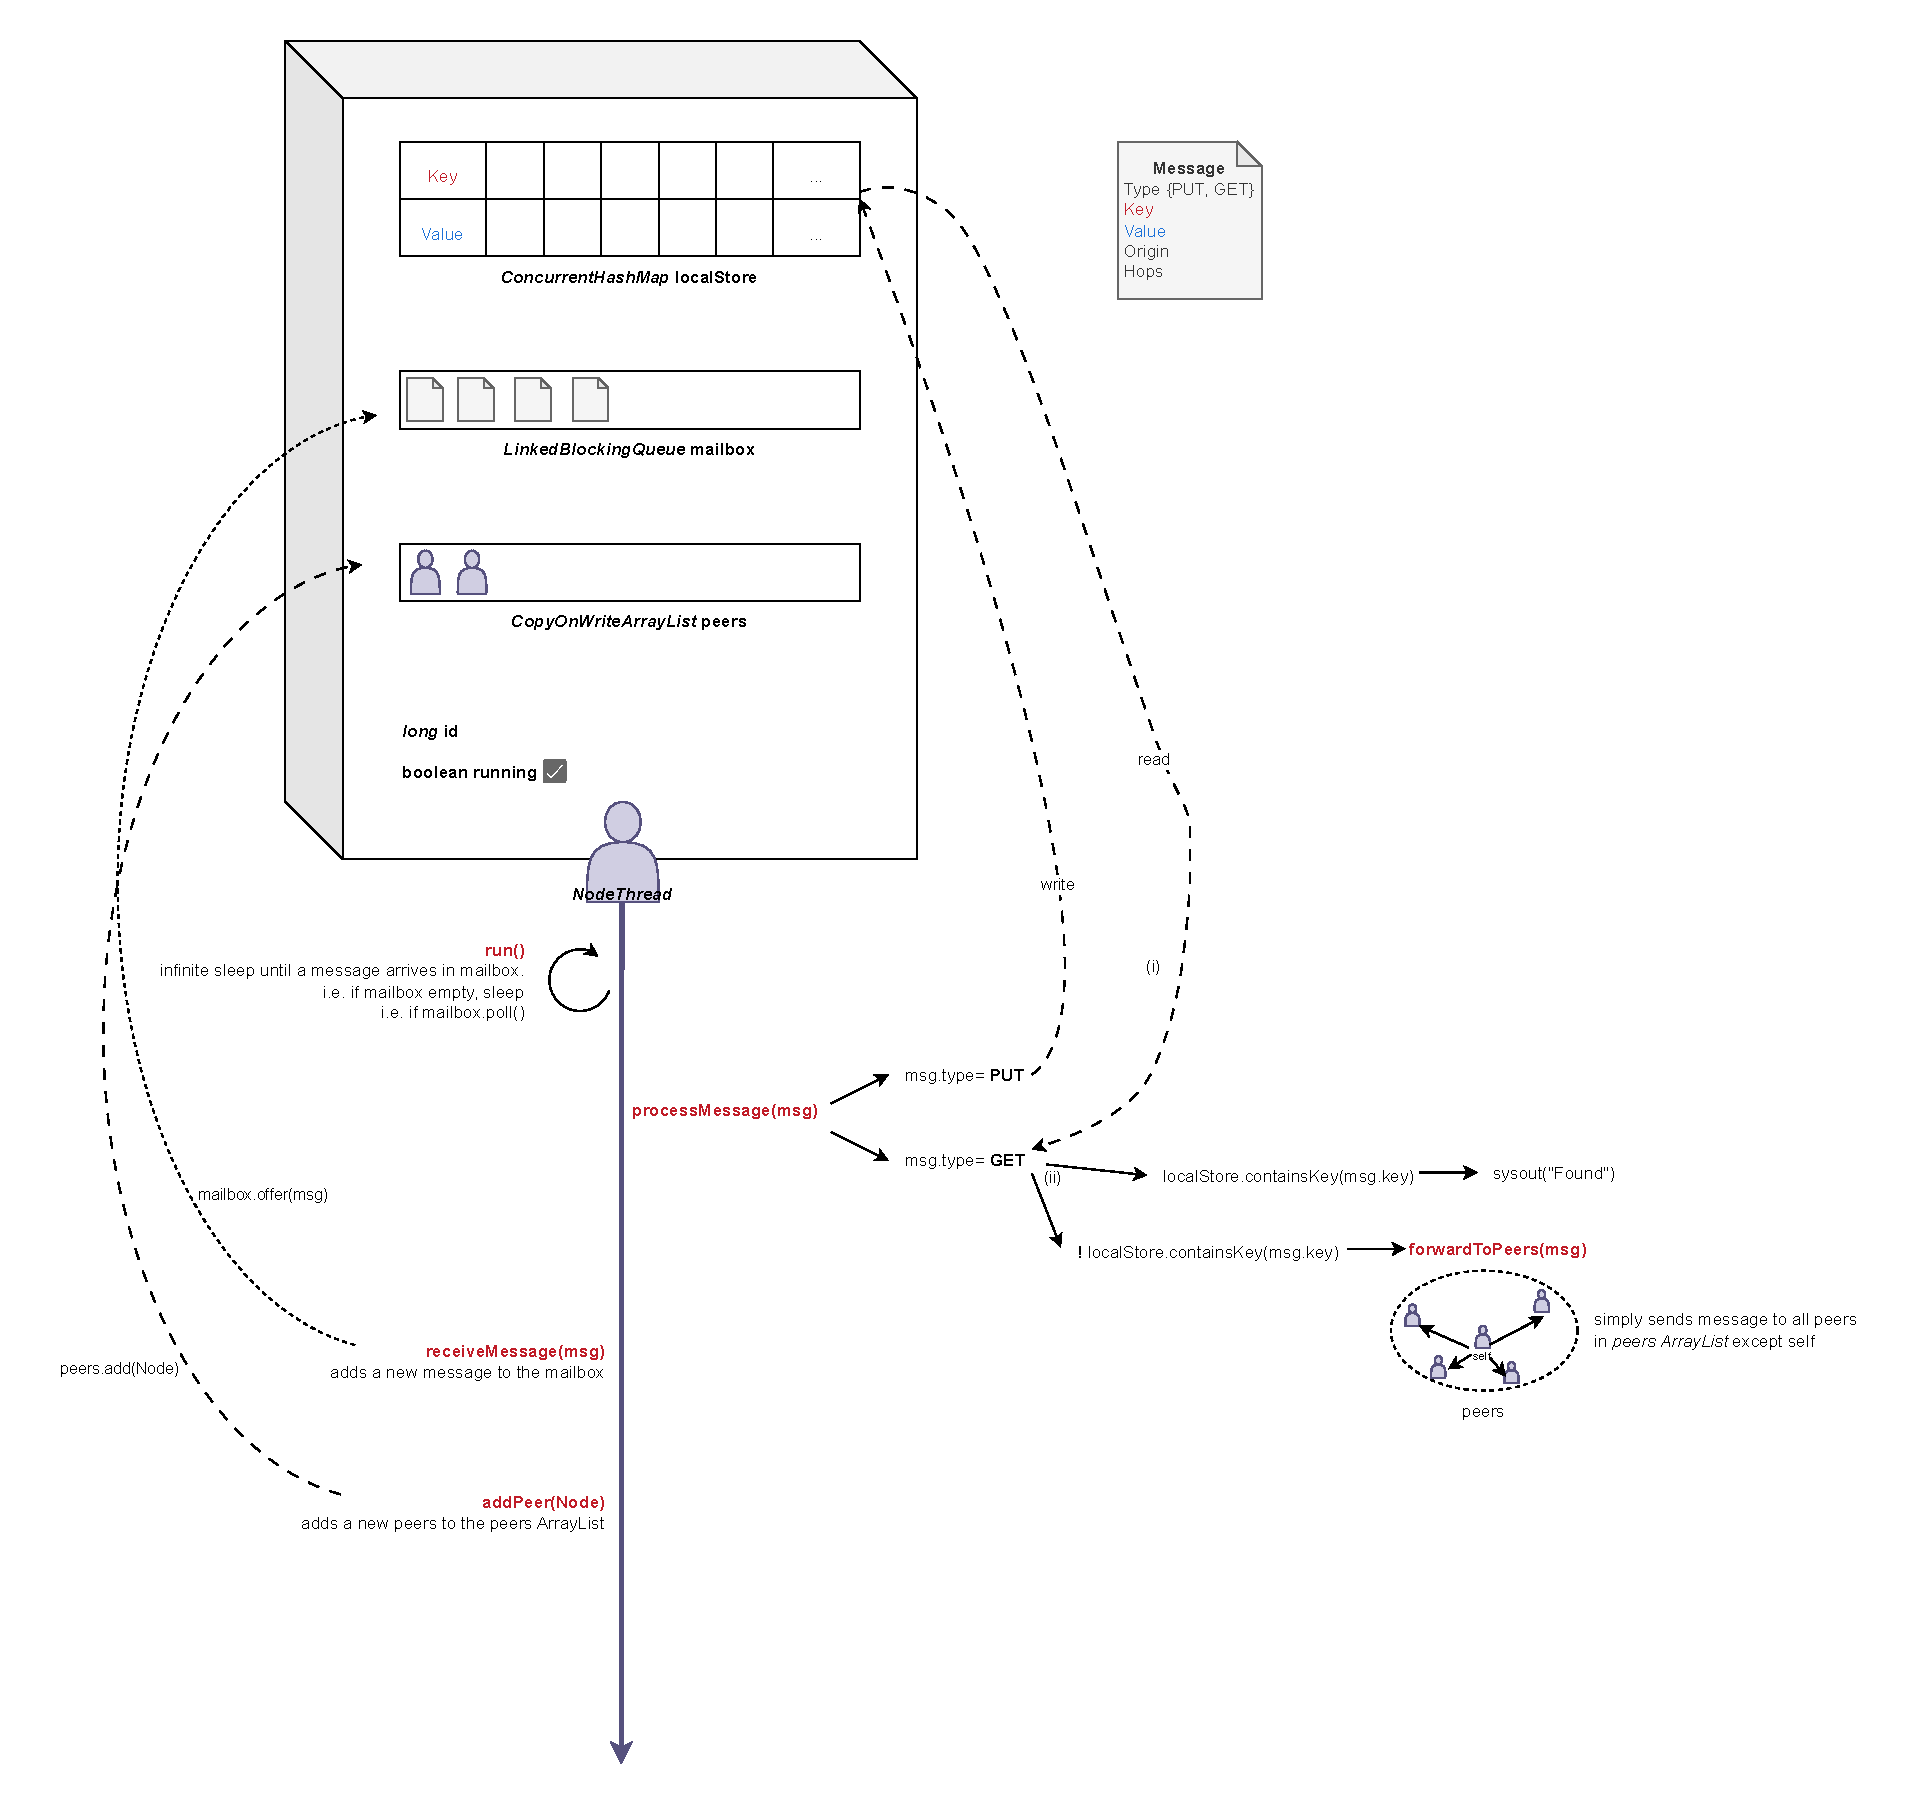
\includegraphics[width=0.8\textwidth]{figures/NodeThread.drawio.pdf}
    \caption{\textbf{Architecture interne et fonctionnement du \texttt{NodeThread}.} Ce diagramme d\'etaille la composition d'un n\oe ud. La fl\`eche verticale symbolise le thread actif, tandis que la bo\^ite 3D repr\'esente l'objet \texttt{Node} avec son \'etat (\texttt{id}, \texttt{running}) et ses structures (\texttt{peers}, \texttt{localStore}). La structure \texttt{Message} est dessin\'ee en gris pour montrer qu'elle est stock\'ee dans la \texttt{mailbox}. Les mots cl\'es Key et Value sont mis en \'evidence pour montrer le transfert d'information du message vers le stockage local. Les fonctions principales sont aussi d\'ecrites : \texttt{run()} maintient le n\oe ud actif, \texttt{receiveMessage()} ajoute les requ\^etes \`a la file, et \texttt{processMessage()} traite la logique m\'etier.}
    \label{fig:node_thread_architecture}
\end{figure}

Pour garantir la stabilit\'e de ce mod\`ele face aux acc\`es concurrents, nous choisissons des structures de donn\'ees sp\'ecifiques :
\begin{itemize}
    \item \textbf{Le Stockage (\texttt{localStore})} : L'utilisation d'une \texttt{ConcurrentHashMap} est indispensable. Elle permet \`a un thread de lire une donn\'ee (\texttt{GET}) pendant qu'un autre message de type \texttt{PUT} met \`a jour la table, \'evitant ainsi les corruptions de donn\'ees.
    \item \textbf{La Liste de Voisinage (\texttt{peers})} : Impl\'ement\'ee via une \texttt{CopyOnWriteArrayList}, elle permet de parcourir les voisins en toute s\'ecurit\'e. Cette structure est optimale car les voisins changent peu apr\`es la phase de d\'ecouverte, mais sont consult\'es \`a chaque transfert de message.
\end{itemize}

\subsection{Le M\'ecanisme de Communication : La Mailbox}
Une fois les n\oe uds actifs, ils communiquent via une \texttt{mailbox} impl\'ement\'ee par une \texttt{LinkedBlockingQueue}. Ce m\'ecanisme permet de d\'ecoupler l'envoi de la r\'eception. Le choix de la m\'ethode d'insertion est ici strat\'egique :
\begin{itemize}
    \item \textbf{L'avantage de \texttt{offer()}} : Contrairement \`a \texttt{add()} ou \texttt{put()}, la fonction \texttt{receiveMessage(msg)} utilise \texttt{mailbox.offer(msg)}. C'est une tentative non-bloquante qui ajoute le message \`a la file sans interrompre l'exp\'editeur. Cela pr\'evient les \textit{deadlocks} (blocages mutuels) o\`u deux n\oe uds s'attendraient ind\'efiniment.
\end{itemize}

\subsection{\'Evolution du Message : Du simple "Sender" \`a l'"Origin"}
La gestion des messages constitue le c\oe ur du routage. L'analyse a montr\'e qu'en relayant un message, le n\oe ud receveur perdait la trace de l'initiateur, rendant la r\'eponse impossible.

Comme l'illustre la Figure \ref{fig:message_evolution}, nous sommes pass\'es d'une structure simple \`a une structure permettant le suivi :

\begin{figure}[H]
    \centering % This centers the group of two images on the page
    
    % --- Image 1: Message v0 (Reduced size) ---
    \begin{subfigure}[b]{0.2\textwidth} 
        \centering
        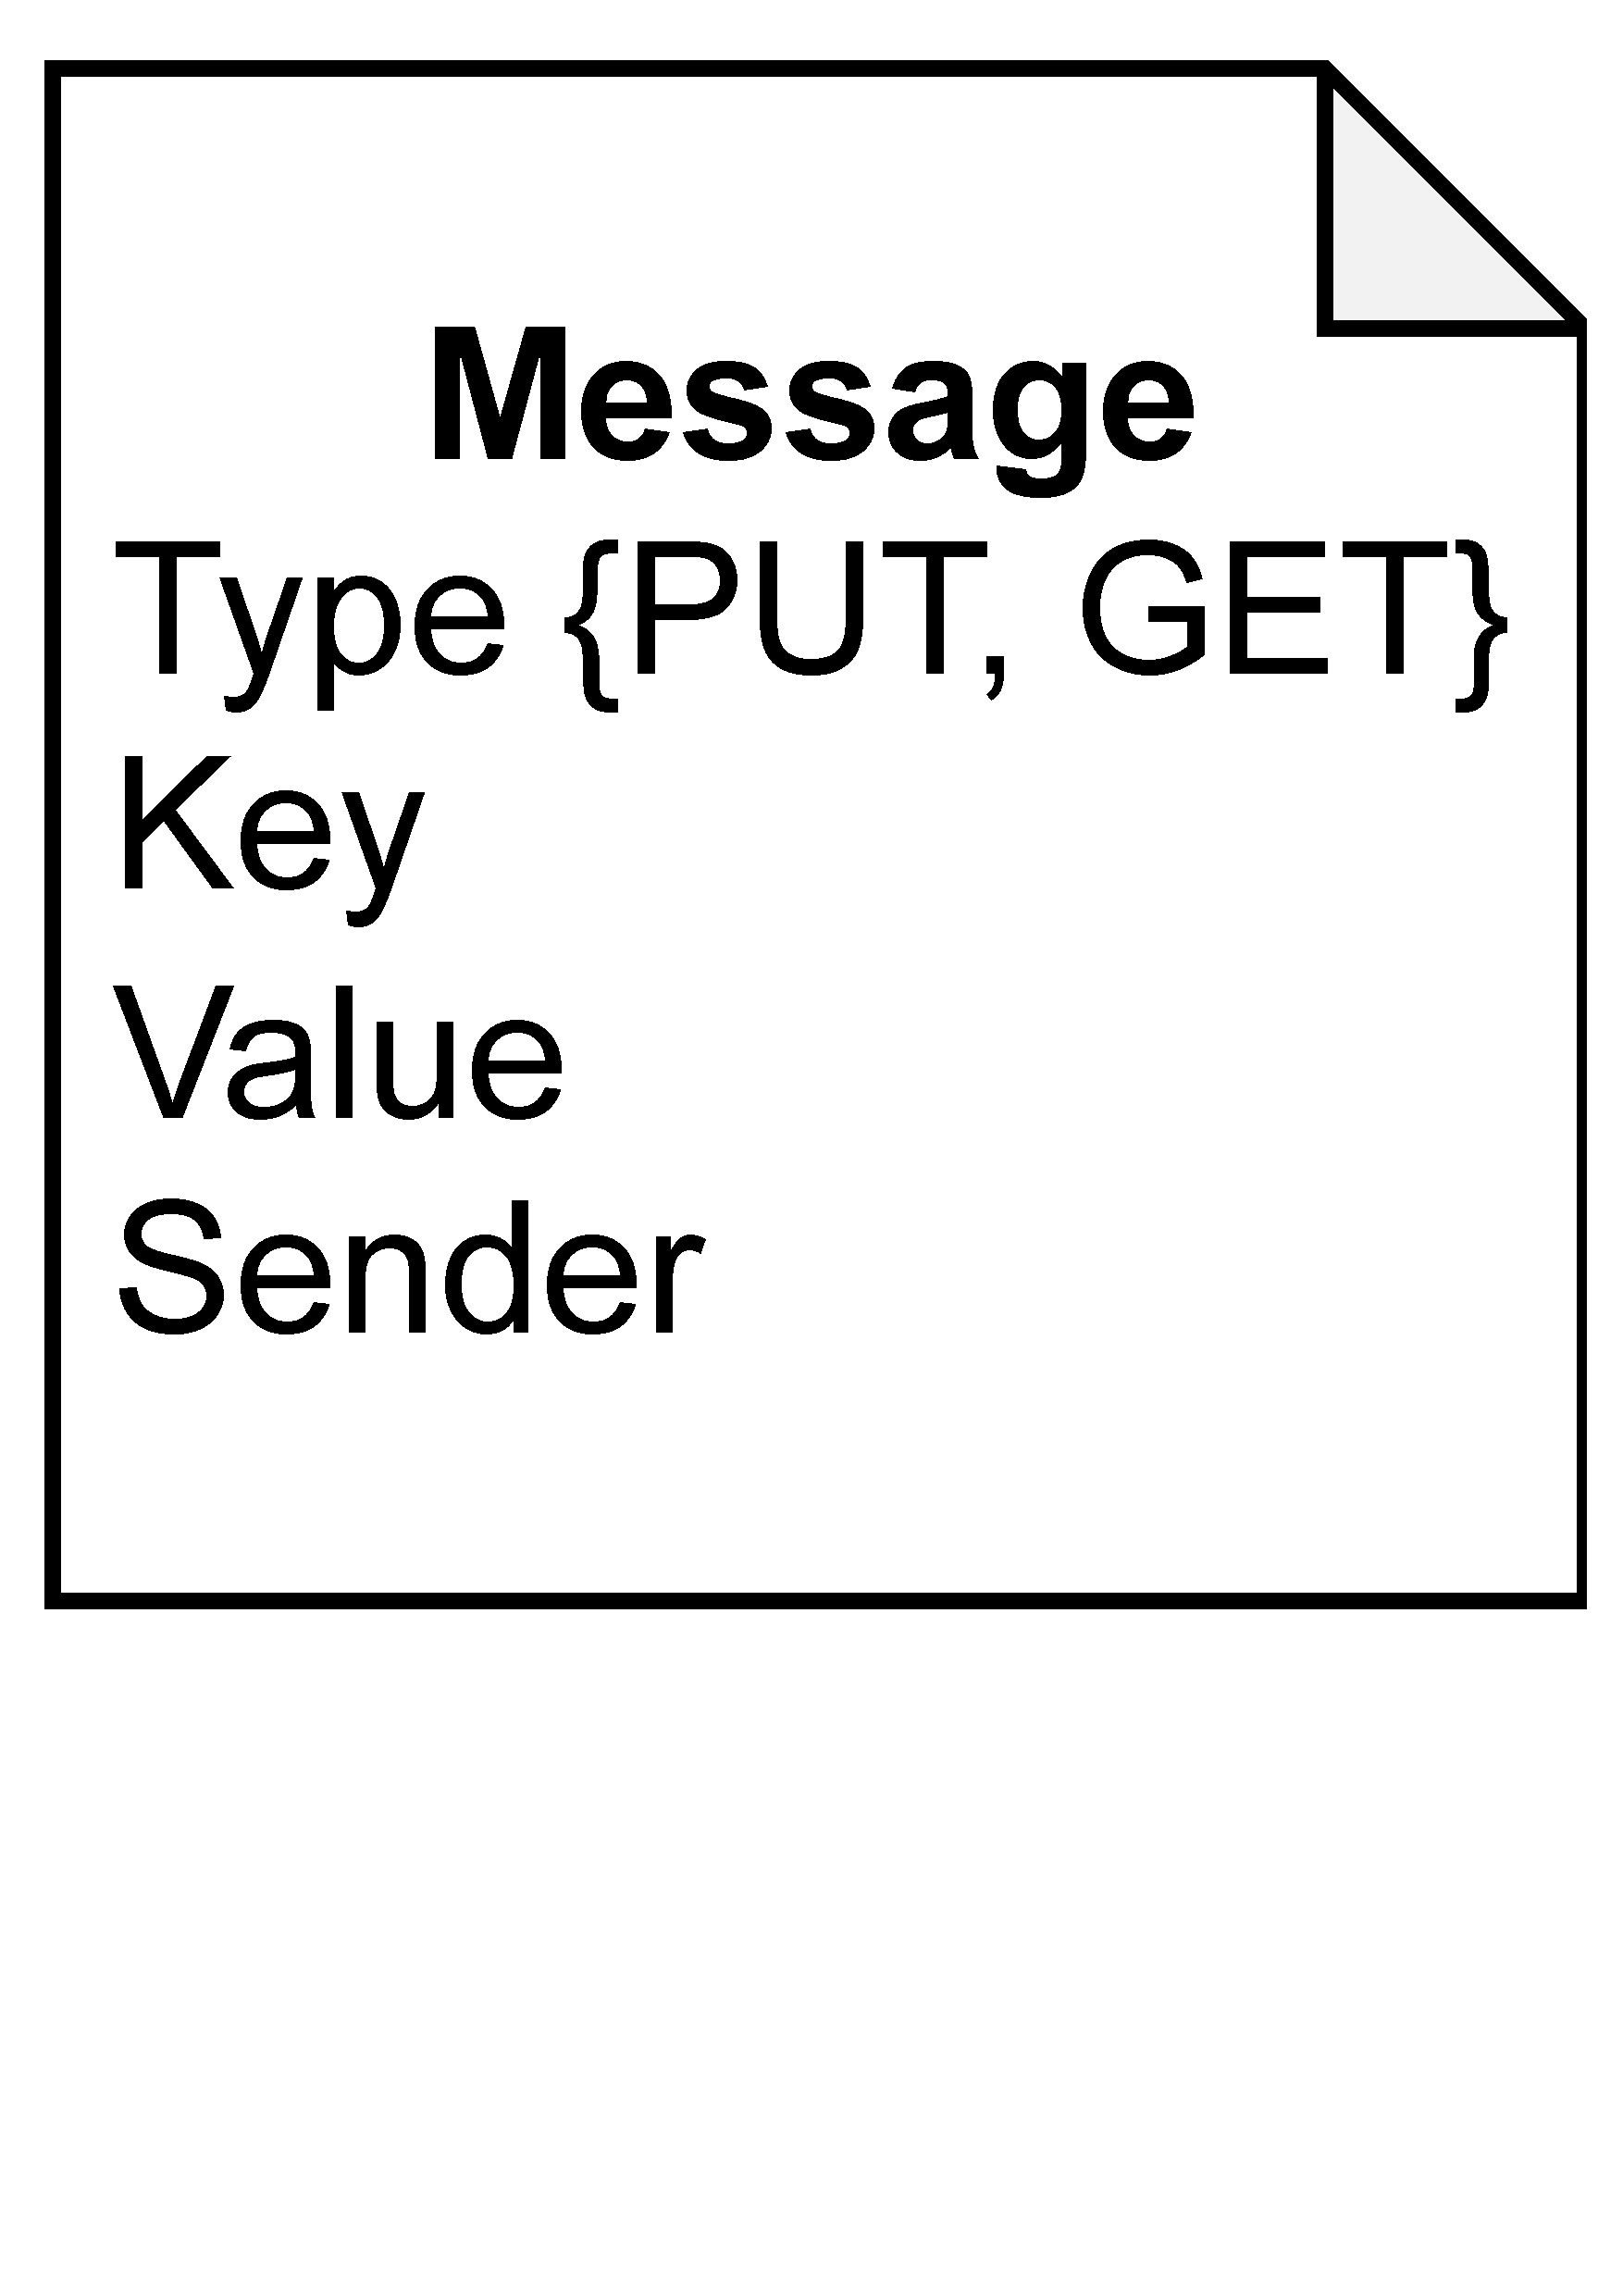
\includegraphics[width=\textwidth]{figures/Messagev0.drawio.pdf}
        \caption{\textbf{v0} : Limit\'e au \texttt{Sender}.}
        \label{fig:msg_v0}
    \end{subfigure}
    %
    \hspace{1cm} % Fixed space between images (keeps them close)
    %
    % --- Image 2: Message v1 (Reduced size) ---
    \begin{subfigure}[b]{0.2\textwidth} 
        \centering
        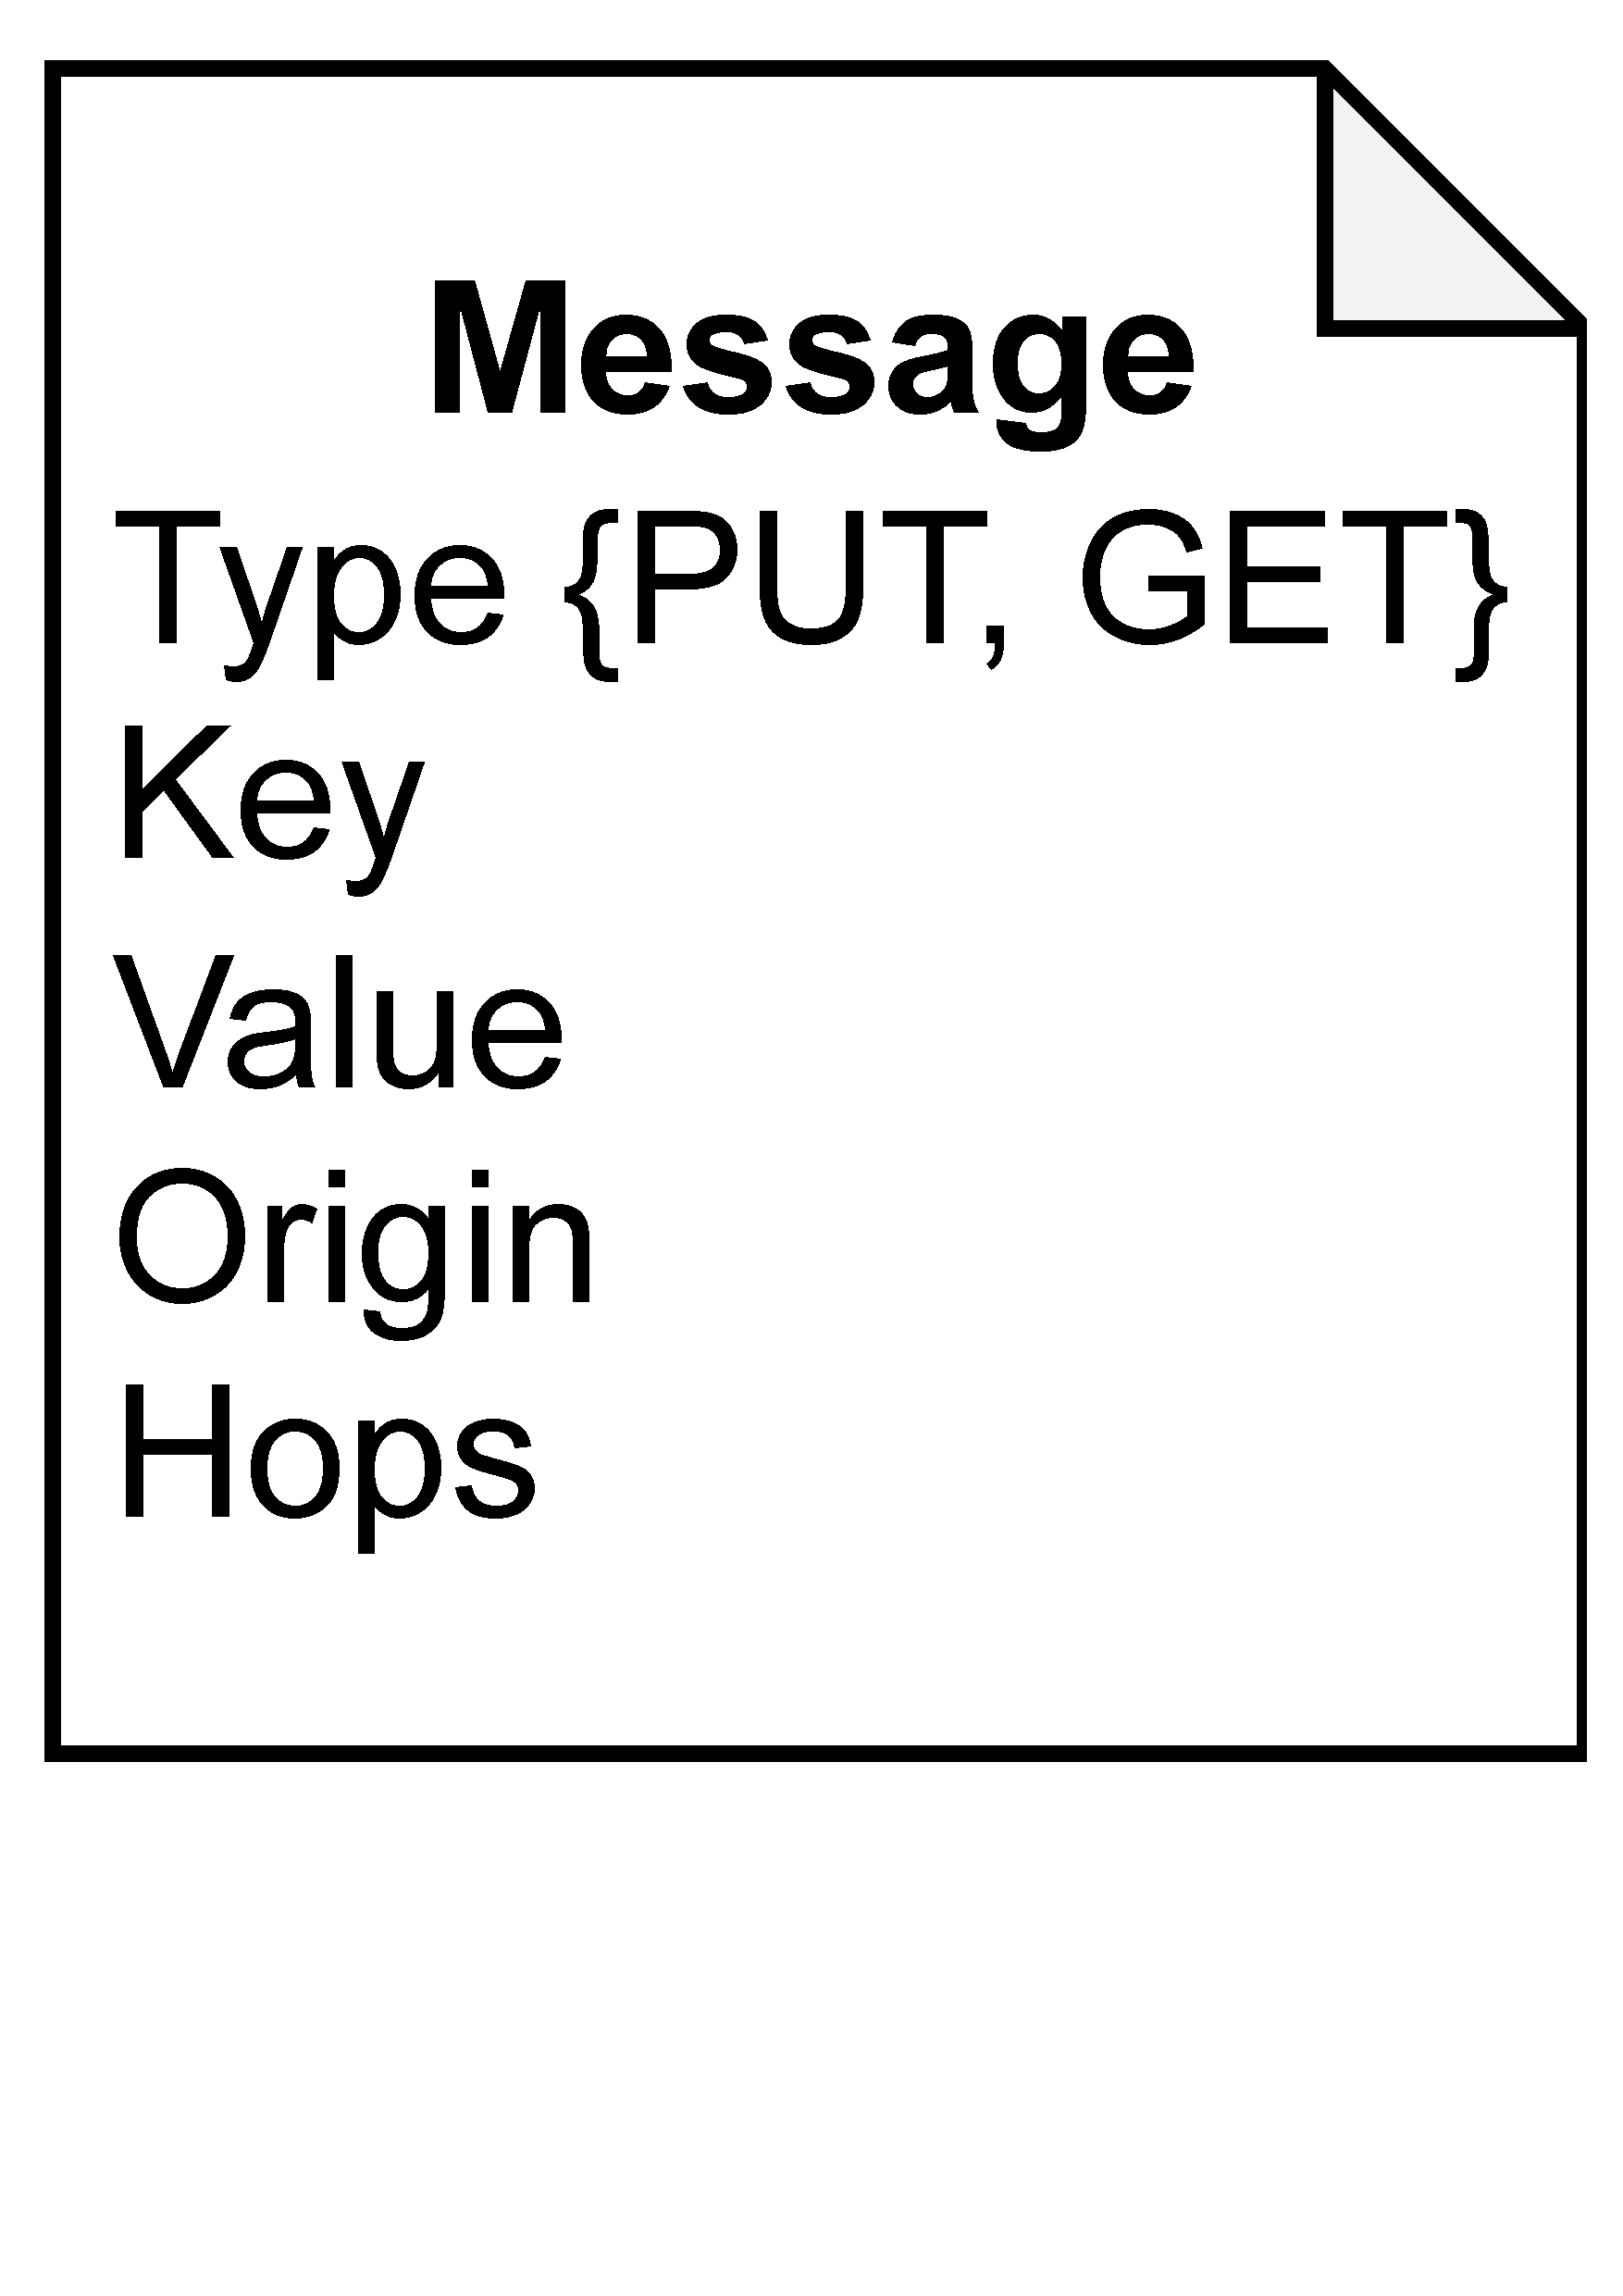
\includegraphics[width=\textwidth]{figures/Messagev1.drawio.pdf}
        \caption{\textbf{v1} : Ajout de \texttt{Origin}.}
        \label{fig:msg_v1}
    \end{subfigure}
    
    \caption{Comparaison de l'\'evolution de la structure du Message.}
    \label{fig:message_evolution}
\end{figure}

Dans la version initiale (\textbf{v0}), le message ne contenait que l'exp\'editeur imm\'ediat. La version actuelle (\textbf{v1}) remplace ce champ par l'\texttt{Origin}. En conservant cette r\'ef\'erence fixe, le message garde son identit\'e tout au long de son parcours.

\subsection{Mesure du parcours et topologie du syst\`eme}
Le \texttt{DHTSystem} orchestre le r\'eseau via deux \'etapes cl\'es : l'ajout de n\oe uds (\texttt{addNode}) et la cr\'eation de liens bidirectionnels (\texttt{buildDiscoveryChain}). Comme le montre la Figure~\ref{fig:dht_system_topology}, cette cha\^ine permet la propagation des messages de proche en proche. Pour diagnostiquer l'efficacit\'e de ce routage, nous int\'egrons un compteur de \texttt{Hops}. \`A chaque transfert vers un pair, ce compteur s'incr\'emente, permettant de d\'etecter les inefficacit\'es ou les recherches trop longues.

\begin{figure}[H]
    \centering
    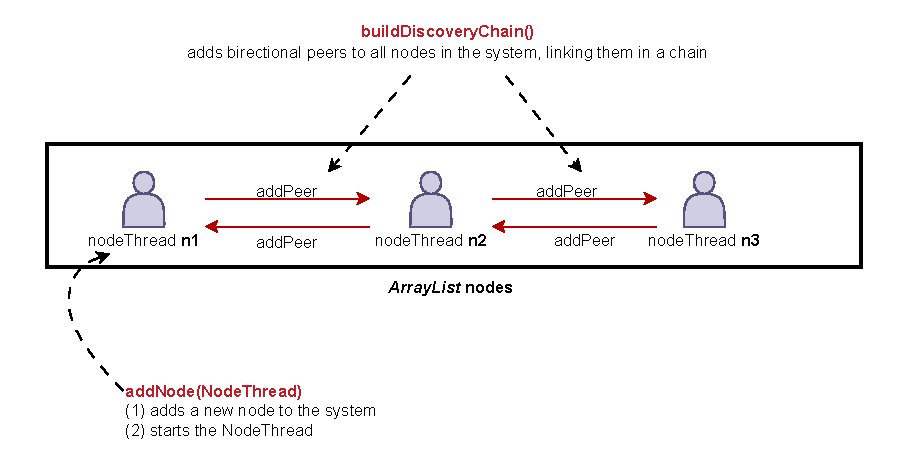
\includegraphics[width=0.8\textwidth]{figures/DHTSystem.drawio.pdf}
    \caption{\textbf{Topologie et initialisation du r\'eseau via \texttt{DHTSystem}.} Ce sch\'ema illustre l'organisation des n\oe uds stock\'es dans une \texttt{ArrayList}. En bas, la fonction \texttt{addNode()} est indiqu\'ee comme responsable de l'ajout d'un nouveau n\oe ud et du d\'emarrage de son thread. En haut, la fonction \texttt{buildDiscoveryChain()} est mise en \'evidence : elle parcourt la liste pour \'etablir des connexions bidirectionnelles entre les n\oe uds voisins. Ces connexions sont mat\'erialis\'ees par les fl\`eches rouges \texttt{addPeer}, transformant la simple liste en une cha\^ine de propagation op\'erationnelle.}
    \label{fig:dht_system_topology}
\end{figure}

\subsection{Analyse des Erreurs et Limites de la V0}

Cette premi\`ere impl\'ementation, bien que fonctionnelle pour les sc\'enarios nominaux, pr\'esente des failles critiques identifi\'ees lors des tests.

\subsection{Erreurs majeures rencontr\'ees}
\begin{itemize}
    \item \textbf{Boucles de recherche infinies} : Si une cl\'e demand\'ee n'existe pas dans le syst\`eme (ex: recherche de "Shape"), le message est transf\'er\'e de n\oe ud en n\oe ud sans jamais s'arr\^eter. Les threads continuent de saturer la file d'attente de leurs voisins ind\'efiniment.
    \item \textbf{Probl\`eme de Flooding} : Actuellement, un n\oe ud propage le message \`a \textit{tous} ses pairs. Dans un r\'eseau plus large, cela provoquerait une explosion exponentielle du nombre de messages, paralysant rapidement les ressources CPU et m\'emoire.
    \item \textbf{Absence de m\'ecanisme de retour} : Lorsqu'un n\oe ud trouve une donn\'ee, il se contente d'afficher "FOUND" dans la console. L'origine de la requ\^ete n'est jamais notifi\'ee formellement par le biais d'un message retour.
\end{itemize}

\subsection{Points d'am\'eliorations pour la V1}
Pour stabiliser le syst\`eme, les \'evolutions suivantes sont prioritaires :
\begin{enumerate}
    \item \textbf{Time To Live (TTL)} : Int\'egrer une limite de sauts au sein de la classe \texttt{Message}. Une fois le compteur \`a z\'ero, le message est supprim\'e, stoppant ainsi les recherches infructueuses.
    \item \textbf{Type RESPONSE} : Cr\'eer un nouveau type de message pour permettre l'acheminement de la valeur trouv\'ee directement vers l'initiateur (\texttt{Origin}).
    \item \textbf{M\'emorisation des requ\^etes} : Faire en sorte que chaque n\oe ud garde en m\'emoire les identifiants des messages d\'ej\`a trait\'es pour \'eviter de relayer plusieurs fois la m\^eme requ\^ete.
\end{enumerate}

\end{document}
